\documentclass[a4paper, 12pt]{book}

\usepackage{cite}
\usepackage{times}
\usepackage{verbatim}
\usepackage{color}
\usepackage{url}
\usepackage{graphicx}
\usepackage{array}
\usepackage{indentfirst}
\usepackage{algorithm}
\usepackage{algpseudocode}
\usepackage{enumitem}
\usepackage{courier}
\usepackage{mfirstuc}
\usepackage{fancyvrb}
\usepackage{amsfonts}
\usepackage{ifmtarg}
\usepackage{amsmath}
\usepackage[mathcal]{euscript}
\usepackage{fixltx2e}
\usepackage[notbib]{tocbibind}
\usepackage[colorlinks=true,linkcolor=black,citecolor=black,filecolor=black,urlcolor=magenta,unicode]{hyperref}
\usepackage{rotating}
\usepackage{hhline}
\usepackage{wallpaper}

\newcommand{\ie}{i.e.,\ }
\newcommand{\eg}{e.g.,\ }
\newcommand{\etc}{etc.}
\newcommand\reffig[1]{\hyperref[#1]{Figure~\ref*{#1}}}
\newcommand\refchap[1]{\hyperref[#1]{Chapter~\ref*{#1}}}
\newcommand\refsec[1]{\hyperref[#1]{Section~\ref*{#1}}}
\newcommand\refalgo[1]{\hyperref[#1]{Algorithm~\ref*{#1}}}
\newcommand\reflst[1]{\hyperref[#1]{Listing~\ref*{#1}}}
\newcommand\reflstline[1]{\hyperref[#1]{line~\ref*{#1}}}
\newcommand\reftbl[1]{\hyperref[#1]{Table~\ref*{#1}}}
\newcommand\refdef[1]{\hyperref[#1]{Definition~\ref*{#1}}}
\newcommand\ThreadTracer{\textsc{ThreadTracer}}
\newcommand\Lockset{\textsc{Lockset}}
\newcommand\Djitp{\textsc{Djit$^{+}$}}
\newcommand\Goldilocks{\textsc{Goldilocks}}
\newcommand\FastTrack{\textsc{FastTrack}}
\newcommand\Eraser{\textsc{Eraser}}
\newcommand\RoadRunner{\textsc{RoadRunner}}
\newcommand\LiteRace{\textsc{LiteRace}}
\newcommand\Pacer{\textsc{Pacer}}
\newcommand\hb{\includegraphics[scale=0.7]{fig/hb}}
\newcommand\mhpr{\includegraphics[scale=0.7]{fig/mhpr}}
\newcommand\usecourier[1]{{\usefont{T1}{courier}{m}{n} {#1}}}
\newcommand\Tracer{\usecourier{Tracer}}
\newcommand\JIT{\usecourier{JIT}}
\newcommand\Rewriter{\usecourier{Rewriter}}
\newenvironment{definition-box}%
	{\begin{description}\addtolength{\itemsep}{-0.5\baselineskip}\addtolength{\itemindent}{3em}}%
	{\end{description}}
\newenvironment{center-figure}%
	{\begin{figure}[htb]\begin{center}}%
	{\end{center}\end{figure}}
\newenvironment{center-table}%
	{\begin{table}[htpb]\begin{center}}%
	{\end{center}\end{table}}

\usepackage{listings}
\usepackage{textcomp}
\lstset{
	language=C++,
	stringstyle=\rmfamily
	commentstyle=\itshape\color[rgb]{0.133,0.545,0.133},
	showstringspaces=false,
	basicstyle=\ttfamily\scriptsize,
	numberstyle=\tiny,
	numbers=left,
	stepnumber=1,
	numbersep=10pt,
	tabsize=2,
	breaklines=true,
	prebreak = \raisebox{0ex}[0ex][0ex]{\ensuremath{\hookleftarrow}},
	breakatwhitespace=false,
  	columns=fixed,
  	upquote=true,
  	extendedchars=true,
%	frame=single,
	xleftmargin=2em,
	xrightmargin=.5em,
	escapeinside={(*@}{@*)},
	mathescape,
}

\usepackage{amsthm}
\newtheorem{mydef-no-caption}{Definition}
\newenvironment{mydef}[1][]%
	{\begin{mydef-no-caption}{\ifnotmtarg{#1}{\textnormal{(\textbf{#1})}~}}}%
	{\end{mydef-no-caption}}

\usepackage{numprint}
\npthousandsep{,}
\npthousandthpartsep{}
\npdecimalsign{.}

\usepackage{tabularx}
\usepackage{multirow}

\usepackage{ntu}
\hypersetup{
	pdfauthor={\authorEN{}},
	pdftitle={\titleEN{}},
	pdfsubject={NTU Master Thesis}
}

\usepackage{setspace}

\usepackage[absolute]{textpos}
\textblockorigin{0mm}{0mm}

\setcounter{tocdepth}{2}

\pagestyle{plain}

\begin{document}

% cover page
\maketitle

% side page, used for printing on spline.
% \makeside

\frontmatter

\hspace*{-6cm}
\begin{textblock}{16}(-0.4, 0)
	\includegraphics{fig/certification.eps}
\end{textblock}
\newpage

\CenterWallPaper{0.25}{fig/ntu_watermark.eps}
\begin{CJK}{UTF8}{nkai}
\CJKhorz
%\makecertification

\onehalfspacing
%\begin{acknowledgementsCH}

\setlength{\baselineskip}{1.5em}
%經過兩年的長跑,攻讀碩士的生涯也終要邁向終點。

%首先我要感謝我的指導教授廖世偉博士,在百忙之中還是不厭其煩的和我討論。他亦師亦友的指導,總讓我學到比所想要的還要多。%
%我要感謝五位口試委員,洪士灝教授、郭大維教授、施吉昇教授、楊佳玲教授以及蔡欣穆教授,因為有他們的批評與指教,這篇論文%
%才能更臻完美。謝謝實驗室的所有同學們,給予我鼓勵和即時的協助。最後,我要感謝我的父母,因為他們的悉心照料讓我能夠%
%無後顧之憂、全心全力的投入於研究。
%
%而在兩年的長跑後,要迎向的,是我人生另一個新的起點。

在這碩士兩年來,最先要感謝的就是我的指導教授廖世偉老師。雖然工作繁重,但總是會盡可能地抽空給予我們協助,%
對我而言,指導教授不像是大家所俗稱的老闆,反而比較像是工作上的夥伴、工作外的朋友。除了課業上的指導外,也關心我們的生涯發展,謝謝老師。\\%

接著要感謝的就是在碩一給我極大鼓勵與幫助的張家榮學長,不論我問什麼問題,總是不厭其煩地耐心指導我。也因為有著老師與學長為榜樣,%
讓我在碩士生涯中,永遠有個需要努力追求的目標。\\%

還要謝謝三位口試委員:蘇雅韻教授、楊佳玲教授、以及黃世勳教授能撥空參加我的口試,也因為有三位口試委員以及指導教授的指點之下,%
才得以完成這篇論文。\\%

最後,感謝父母、家人的全力支持,讓我衣食無憂地將心思全力投注在研究上;感謝實驗室的同學、學弟們,研究課題上的討論讓我學習到許多,而課業外%
因有著你們的陪伴也讓我研究所生活多采多姿。\\%

結束了十八年的學涯後,期許自己能為我們的社會、國家貢獻一些力量。%
\end{acknowledgementsCH}

\begin{abstractCH}

\setlength{\baselineskip}{1.5em}
為了追求 (1) 效能; (2) 可移植性; (3) 使用性,Google 在 Android 3.0 的版本中推出了 RenderScript。我們延伸其功能,使之可遠端化。具體一點的說法,我們透過網路接口傳送 RenderScript 命令到遠端圖形引擎上。請注意,在此所提到的遠端引擎可以是在同一裝置或是遠端裝置之上。

我們的貢獻分為兩個部分:\\
        \\首先,我們讓 RenderScript 現有的先進先出佇列可以連網。我們建構了一個轉運層以實現網路功能抽象化。\\
        \\第二,透過把指令傳送到遠端引擎之上,我們可以重新在該引擎上執行所接收而來的命令。視不同型態的遠端引擎而定,重新執行命令的動作可能會需要把 RenderScript 的命令對應到 egl、glx、agl、或是 wgl。其分別對應於不同的平台,依序為 Android, Linux, Mac OS, Windows。在本論文中,我們將敘述對應到 egl 的實作細節。

\end{abstractCH}

\begin{abstractEN}

Google introduces RenderScript as part of Android 3.0 for the following reasons: (1) Performance;  (2) Portability; and (3) Usability. We extend it to make it remote-able. Specifically, we send RenderScript commands through a socket to a remote graphics engine. We use the term, remote engine, to refer to the engine on the same device or on a remote host. 

Our contribution is two-fold. First, we make the existing FIFO queues in RenderScript network-ready. We build the transport layer to facilitate the networking abstraction. Second, we replay the commands on the remote engine by materializing the commands on top of a remote engine. Depending on the type of remote engines, the replay may need to map RenderScript commands to egl, glx, agl, or wgl. They are for Android, Linux, Mac OS, or Windows, respectively. We demonstrate the egl-mapped implementation in this thesis.

\end{abstractEN}

\begin{comment}

\category{D2.4}{Software}{Software Engineering --
Software/Program Verification} 
\category{D2.5}{Software}{Software Engineering -- 
Testing and Debugging}
\category{F3.1}{Theory of Computation}{Logics and Meanings of Programs -- 
Specifying and Verifying and Reasoning about Programs.}

\terms{Algorithms, Design, Verification.}

\keywords{OpenMP, GCC, LLVM, data race, multithread, dynamic analysis, static analysis.}

\end{comment}

\tableofcontents
\end{CJK}
\listoffigures
\listoftables

\mainmatter

\renewcommand{\arraystretch}{2.0}
\doublespacing
% input your thesis here
\chapter{Introduction}
\label{c:intro}

% Background

%# of mobile phone users
With the increasing adoption of smartphones~\cite{increasing-phones}, more and more software developers are interested in building mobile applications for smartphones~\cite{attract-game-developer}. Among the various types of mobile applications, game is the most popular. According to \cite{gamepercent1} and \cite{gamepercent2}, by 2010, about 58 percent of the applications in the biggest mobile application store (i.e., Apple's App Store) are games.

However, on Google's Android platform, existing tools for game development are still not perfect. For instance, developers need to deal with the low-level details of JNI (Java Native Interface) calls such as method signature when using Android NDK (Native Development Kit) ; are not able to use GLSL (OpenGL Shading Language) for mathematical computation; and are more difficult to build an application with satisfying performance by using Android SDK (Software Development Kit).

More specifically on the limitation, Java interacts poorly with most current 3D APIs: (1) The interface of Java and native GL is not ideal; (2) Lots of copies or translations needed. Current 2D application performance is not what we would like: (1) Walking through the view hierarchy is slow; (2) Applications need to be called each time we render , e.g., \textit{onDraw()}.; (3) Skia is a poor fit for GL acceleration; (4) We are not in a position to scale to multiple threads; and more importantly, (5) we need 3D apps, Skia performance on larger size screen is unacceptable.

To overcome above limitations, Google introduces a framework, \RS{}\cite{renderscript-part1}, in Android SDK 3.0 named Honeycomb. (For simplification, we use RS and \RS{} interchangably in this thesis.) 

\RS{} aims to provide high performance 3D rendering and mathematical computation at the native level, which targets for the following goals: (listed from most to least important) \cite{renderscript-part2}
\begin{itemize}
	\item \textbf{Portability} ─{} Application code needs to be able to run across all devices with different hardware, and be able to fully utilize the capability of various hardwares. For example, ARM currently comes in several variants: with and without VFP, with and without NEON, and with various register counts. Beyond ARM, application code should be able to run on other CPU architectures such as x86, or even run on a GPU or a DSP.
	\item \textbf{Performance} ─{} The second goal is to get as much performance as possible under the requirement of portability. 	
    \item \textbf{Usability} ─{} The third goal is to simplify development as much as possible by offloading the heavy lifting of interfacing with a native graphics API while retaining full application control. Where possible we automate steps to avoid hand-written glue code and other developer-side busy work.
\end{itemize}

% Propose

There are two kinds of \RS{}s: compute and graphics. A compute \RS{} does not do any graphics rendering while a graphics \RS{} does.

A \RS{} application comprises both Java codes and native codes. Similar to other Android applications, the Java code in a \RS{} application uses Android SDK API. The native code, or the RS script in other words, is actually written in a C99-standard C language with extensions such as vector operations, function overloading, and rsForEach() parallelization. Note that a \RS{} application contains at least one RS script, you write and save it to a .rs file in your project. 
The communication between Java codes and native codes is through JNI function calls. Simply stated, there are \textbf{two layers and one bridge in between}:
\begin{itemize}
\item Android \textit{System Layer} (\textbf{Java Framwork}, i.e., \textit{framework.jar}) : That is, traditional framework APIs, which include the \RS{} APIs in \verb|android.renderscript|. \Client{} handles things such as the Activity lifecycle management of your Android application and communicates with the native \RS{} code via \textit{Bridge}.
\item \textit{Native Layer} (Codes stored in the \textbf{native .rs files}) : \Core{} is responsible for doing intensive computing and graphics rendering tasks. \Core{} returns the result to \Client{} through \Bridge{}. 
\item \textit{Bridge} (\textbf{JNI}, i.e., \textit{librs\_jni.so}, and \textbf{reflected Java classes}) : \Bridge{} deals with the communication between the above two layers. The Android build tools automatically generate the classes for \Bridge{} during the build process. \RS{} uses lockless FIFO (First In and First Out) command queue to communicate between layers. Figure \ref{fig:Java-C-communicate-flow} shows the flow of communication.
\end{itemize}

\begin{center-figure}
    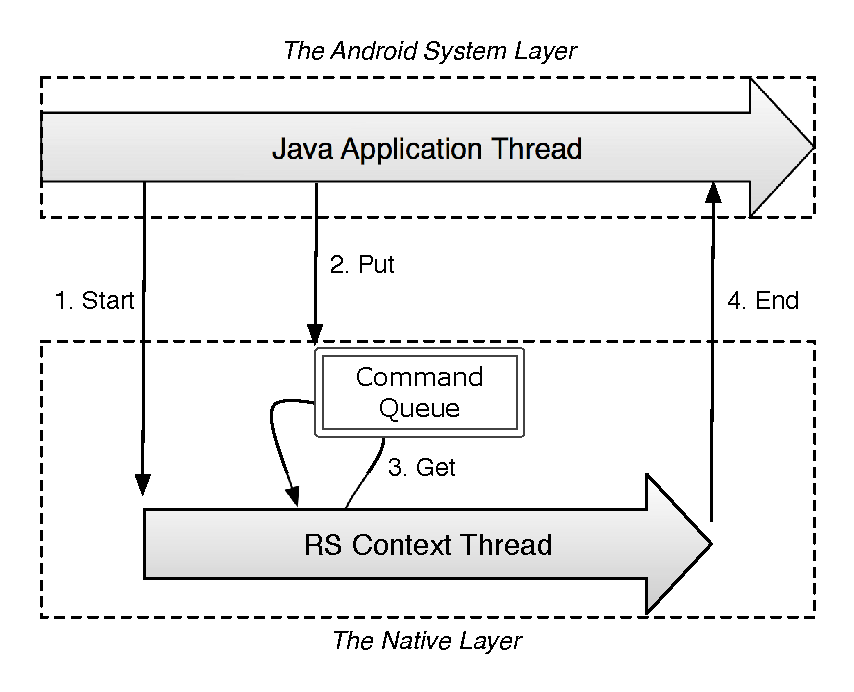
\includegraphics[scale=0.8]{fig/LocklessFifo.eps}
    \caption{Communication between Java and RS code}
    \label{fig:Java-C-communicate-flow}
\end{center-figure}

As Figure \ref{fig:Java-C-communicate-flow} shows, minimal work is done in the application thread, and no native drawing calls are directly from Java application codes. (i.e., All drawing calls are invoked from \Core{}) The RS native thread does heavy lifting: screen can be refreshed without a callback to the Java application thread.

\begin{enumerate}[label=Step \arabic*., font=\sffamily\bfseries]
\item When a \RS{} application is launched, \Client{} creates a Java application thread. After being initialized, the Java application thread notifies \Core{} to create an RS context thread and establish the command queue via \Bridge{}. 
\item Both computing and rendering are done at \Core{} and UI events are handled in the \Client{}. Once the Java application thread receive an event, it puts the commands for computation or rendering into the FIFO command queue.
\item If all of the conditions are met, RS context thread will keep polling the command queue until getting a command. While getting a command, the RS context thread executes the command in \Core{}. (See Chapter \ref{ss:ThreeCondition})
\item As the RS context thread receives a destory signal, the control is handed over to \Client{}.
\end{enumerate}
We will discuss the flow in more details in Chapter \ref{c:OverviewRS}.

Although the \RS{} framework is a major improvement in development of fancy visual effects and other computing intensive application, developers may find it difficult to develop Renderscript applications due to the absence of a debugger or an emulator. Although Google does provide an emulator for Android Honeycomb, it is only starting to support OpenGL ES 2.0, which is required to run \RS{} applications. 

For reducing the complexity of development and debugging, we need a mechanism which can replay and execute \RS{} commands on the remote engine. To accomplish the objective, we propose the \RRS{} architecture in this thesis. The main idea of the \RRS{} architecture consists of two steps. Based on the architecture showed in Figure \ref{fig:Java-C-communicate-flow}, first, we extend \RS{} to make it remote-able. To acheive this, we build a \Transport{} on the top of \Core{}. \Transport{} takes care of sending commands of a local \RS{} system to a remote \RS{} system. Figure \ref{fig:transport-layer} below illustrates that.

\begin{center-figure}
    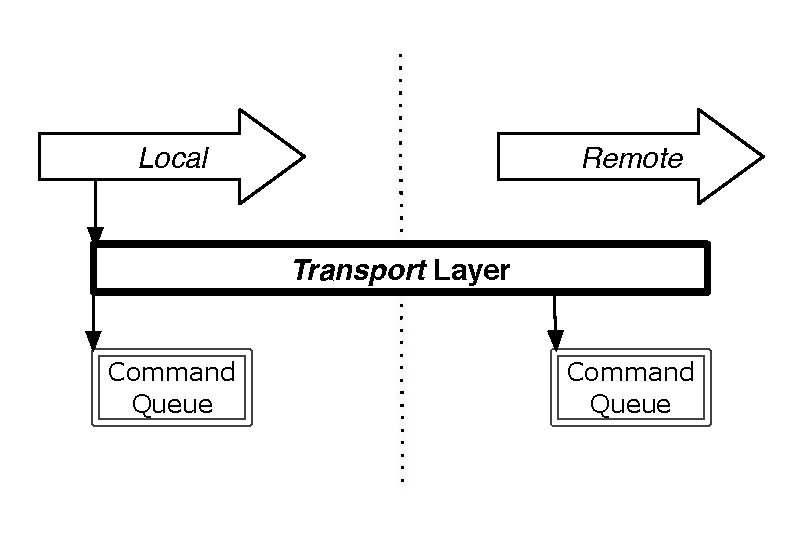
\includegraphics[scale=0.8]{fig/TransportLayer.eps}
    \caption{Transport Layer}
    \label{fig:transport-layer}
\end{center-figure}

Second, we replay the commands on the remote engine by materializing the commands on top of a remote engine. Depending on the type of remote engines, the replay may need to map \RS{} commands to egl, glx, agl, or wgl\footnote{They are OpenGL interfaces for Android, Linux, Mac OS, and Windows, respectively.}. Note that both rendering and computing commands are played in individual engine so that we could leverage the hardwares on the remote engine. The egl-mapped implementation is demonstrated in this thesis.
%Any smart device is just like a personal-cloud. After the authentication, we could do the above ones by sending commands to each other.
With \RRS{}, we could send the commands from emulator and replay it on the remote host. In this scenario, the remote host is local machine. In our implmentaion, extended \RS{} runtime could enable the debugging option by setting the property via ADB (Android Debugging Bridge).

Additionally, \RRS{} has the potential to be the foundation of many other applicaiotns in addition to debugging, such as remote controlling, collaborating tools, multi-player games, remote monitoring, and etc. 

The rest of the paper is organized as follows. Chapter 2 describes related works. As a background knowledge, Chapter 3 goes through the existing design and implementation of \RS{} system. Chapter 4 illustrates our design of \RRS{}. Chapter 5 discusses the egl-mapped implementation for \RRS{}. Finally, Chapter 6 concludes the thesis and presents the future works.

\chapter{Background of Dynamic Data Race Detection Algorithm}
\label{c:background}

% Use happens-before instead of lockset
Data race detection especially \textit{precise} (no false positives) data race detection is useful. Static techniques for detecting data race needs to be conservative thus often contains bunch of false alarms in their result set. Dynamic techniques based on \Lockset{} algorithm verify whether the program execution conforming to the \textit{lock discipline}. For example, \Eraser{}~\cite{Savage:1997p280} reports there's a race if a shared variable accessed in the program execution isn't protected by some locks. \Lockset{} algorithm based detectors provide better coverage while lose the precision since they don't take care of the \textit{synchronization events} other than the lock. Detectors based on \textit{happens-before} relation~\cite{Lamport:1978p527} however, are usually precise. They combine the program order and synchronization events to reason the `happens-before' relation between access operations. If the reasoning fails, that is, these two operations cannot be ordered by the happens-before relation, there's a possibility that they may be executed concurrently. Since the precise dynamic data race detection is important as we mentioned before, we choose happens-before based algorithm for our data race detector.

The following sections describes the happens-before relation and its implementation using vector clock. Two algorithms \Djitp{} and \FastTrack{} are then introduced in \refsec{s:DJIT+} and \refsec{s:FastTrack} based on vector clocks, respectively.

\section{Happens-Before Relation}
An operation $A$ at thread $t_A$ \textit{happens-before} $B$ at thread $t_B$ denoted as $A$\hb{}$B$ holds if one of the followings is true:
\begin{itemize}
	\item \textbf{Program Order} --- $t_A = t_B$ and $A$ precedes $B$ in the program source code.
	\item \textbf{Synchronization Events}
	\begin{itemize}
		\item \textbf{Lock} --- $B$ is a lock \textit{acquire} operation on lock object $L$ after the lock \textit{release} operation $A$ on $L$.
		\item \textbf{Fork} --- $A$ is a \textit{fork} operation that forks a new thread $t_B$.
		\item \textbf{Join} --- $A$ is a \textit{join} operation that blocks $t_A$ until thread $t_B$ terminates.
	\end{itemize}
	\item \textbf{Transitive} --- $\exists C$ at $t_C$ such that $A$\hb{}$C$ and $C$\hb{}$B$.
\end{itemize}

If there're two operations $A$ and $B$ such that neither $A$\hb{}$B$ nor $B$\hb{}$A$ holds, then it's possible that $A$ and $B$ are concurrent operations. If $A$ and $B$ perform operation on the same memory location (\eg{} on the same shared variable) and one of them is write, the program is said to contain data race.

\section{Vector Clocks}
\label{s:DJIT+}
Vector clock~\cite{Mattern:1988p817} is one of the algorithms for reasoning the happens-before relation between the events. Before the review of the vector clock-based data race detection algorithms, we define two operators for vector clock. A vector clock $VC$ is an array in which each element $VC(t)$ records the clock values of thread $t$ and:
\begin{definition-box}
	\item $VC_1 \ll VC_2 \iff \forall t, VC_1(t) \le VC_2(t)$
	\item $VC_3 \gets VC_1\,\sqcup\,VC_2: \forall t, VC_3(t) \gets max(VC_1(t), VC_2(t))$
\end{definition-box}

Each thread then keeps a vector $C_t$ such that for any thread $u$, $C_t(u)$ records the clock for the last operation of thread $u$ that happens before the current operation of thread $t$. Each lock object $m$ also keeps a vector clock $L_m$ for the purpose of the synchronization the clock vector between thread $t$ and $u$ when $u$ acquires the lock $m$ after the $t$ releases it. Each shared variable $v$ keeps two vector clocks $W_v$ and $R_v$. $W_v(t)$ and $R_v(t)$ records the clocks of the last write and read to $v$ by $t$, respectively.

The \Djitp{}~\cite{Pozniansky:2003p263}, a vector clock-based data race detection is then summarized as follows:
\begin{algorithm}
	\caption{\Djitp{} algorithm}
	\begin{algorithmic}[1]
		\Procedure{Fork}{$t,u$}\Comment{When thread $t$ forks a new thread $u$}
			\State $C_u \gets C_u\,\sqcup\,C_t$
			\State $C_t \gets C_t + 1$
		\EndProcedure
		\Statex
		\Procedure{Join}{$t,u$}\Comment{When thread $t$ blocks until the termination of thread $u$}
			\State $C_t \gets C_t\,\sqcup\,C_u$
			\State $C_u \gets C_u + 1$
		\EndProcedure
		\Statex
		\Procedure{Acquire}{$m,t$}\Comment{When thread $t$ acquires the lock $m$}
			\State $C_t \gets C_t\,\sqcup\,L_m$
		\EndProcedure
		\Statex
		\Procedure{Release}{$m,t$}\Comment{When thread $t$ release the lock $m$}
			\State $L_m \gets C_t$
			\State $C_t \gets C_t + 1$
		\EndProcedure
		\Statex
		\Procedure{Read}{$v,t$}\Comment{When thread $t$ reads shared variable $v$}
			\If{\textbf{not} $W_v \ll C_t$}
				\State \Call{Error}{``write-after-read race''}
			\EndIf
			\State $R_v(t) \gets C_t(t)$
		\EndProcedure
		\Statex
		\Procedure{Write}{$v,t$}\Comment{When thread $t$ writes shared variable $v$}
			\If{\textbf{not} $W_v \ll C_t$}
				\State \Call{Error}{``write-after-write race''}
			\EndIf
			\If{\textbf{not} $R_v \ll C_t$}
				\State \Call{Error}{``read-after-write race''}
			\EndIf
			\State $W_v(t) \gets C_t(t)$
		\EndProcedure
	\end{algorithmic}
\end{algorithm}

\Djitp{} algorithm is \textit{sound} and \textit{precise}. However, it's an $O(n)$ time and space algorithm (where $n$ is proportional to the number of threads in the system). It performs $O(n)$ time operations upon the synchronization event (\eg{} lock acquire and release) and variable access.

\section{\FastTrack{} Algorithm}
\label{s:FastTrack}
\FastTrack~\cite{Flanagan:2009p3} subsequently improves the \Djitp{} from generally $O(n)$ to $O(1)$ time and space \textit{in most time}. It's still \textit{sound} and as \textit{precise} as \Djitp{}. This is achieved by the observation that there's no need to \textit{always} record entire vector clocks $W_v$ and $R_v$ for each variable $v$. Assume we guarantee to report the first data race on $v$. When a variable $v$ is accessed and program remains race-free in the meantime, all previous \textit{writes} should be \textit{totally ordered}\footnote{Because $W_v \ll C_u$ holds for any thread $u$ that accessed $v$.}. Therefore, only the \textit{latest clock} of the write on $v$ need to be checked. $W_v$ then reduces to an \textit{epoch} and the check performed on $W_v$ becomes $O(1)$ time. An epoch $c@t$ is \textit{a scalar} which records only thread $t$ and its clock value $v$.

Unlike $W_v$, $R_v$ cannot simply becomes an epoch since reads are not guaranteed to be totally-ordered even in a race-free program. That is, a write to $v$ may cause race with the any previous reads to $v$ not just the last one. However, time and space complexity still can be reduced by using the epoch instead of the keeping complete vector clocks for $R_v$ as possible as we can. \reffig{fig:FastTrack_read} shows how the representation of $R_v$ being changed. The \textit{empty state} is the initial state of the $R_v$. It's usually an epoch containing the minimum clock values. The state always returns to the empty state after the write to $v$. This is because if the write access doesn't cause data race with previous reads, these previous reads should also \textit{not} cause data races with writes afterward. We can then stop tracking $R_v$ and safely discard past read history by resetting the state to empty state. After the first read by thread $t$ in empty state, the state transits to the \textit{epoch state}. In this state, $R_v$ is represented by an epoch $c@t$ and all subsequent reads by the same thread $t$ only cause an update on $c$. Once there's another thread $t'$ with clock value $c'$ where $t' \not= t$, the state becomes \textit{vector clock} state. $R_v$ becomes a vector clock where $R_v(t) = c$ and $R_v(t') = c'$. Any later read to $v$ by thread $t''$ with clock value $c''$ will update $R_v(t'')$ to $c''$.

\begin{center-figure}
\includegraphics[scale=0.9]{fig/FastTrack_read.eps}
\caption{State transition of the representation of $R_v$}
\label{fig:FastTrack_read}
\end{center-figure}

We define some operators between vector clock $VC$ and an epoch $E = c@t$:
\begin{definition-box}
	\item $E \ll VC \iff E.c < VC(E.t)$
	\item $E =_t VC \iff E.t = t$ and $E.c = VC(t)$
	\item $VC \gets E: VC(E.t) \gets E.c$
	\item $E \gets_t VC: E.t \gets t$ and $E.c \gets VC(t)$
\end{definition-box}

\refalgo{a:FastTrack_pseudocode} shows the pseudo code of \FastTrack{} algorithm. We implement \FastTrack{} on the top of \ThreadTracer{} depicted in the following chapter and use it as default approach to dynamically detect the data races in our detector.

\begin{algorithm}
	\caption{\FastTrack{} algorithm}
	\label{a:FastTrack_pseudocode}
	\begin{algorithmic}[1]
		\State \textbf{Initial:} 
		\State \hspace{1.5em} $W_v \gets$ \textit{an epoch contains minimum clock value}
		\State \hspace{1.5em} $State(R_v) \gets$ \textit{initial state}
		\Statex
		\Procedure{Read}{$v,t$}
			\If{$State(R_v) =$ \textit{epoch state} \textbf{and} $R_v =_t C_t$}
				\State \Return\Comment{No action needed for same epoch}
			\EndIf
			\If{\textbf{not} $W_v \ll C_t$}
				\State \Call{Error}{``write-after-read race''}
			\EndIf
			\If{$State(R_v) =$ \textit{initial state}}
				\State $State(R_v) \gets$ \textit{epoch state}
				\State $R_v \gets_t C_t$
			\ElsIf{$State(R_v) =$ \textit{epoch state}}
				\If{$R_v.t = t$}
					\State $R_v.c \gets C_t(t)$
				\Else
					\State $oldR_v \gets R_v$
					\State $State(R_v) \gets$ \textit{vector clock state}\Comment{$R_v$ becomes a vector clock}
					\State $R_v \gets oldR_v$
					\State $R_v(t) \gets C_t(t)$
				\EndIf
			\Else\Comment{$State(R_v) =$ \textit{vector clock state}}
				\State $R_v(t) \gets C_t(t)$
			\EndIf
		\EndProcedure
		\Statex
		\Procedure{Write}{$v,t$}
			\If{$W_v =_t C_t$}
				\State \Return\Comment{No action needed for same epoch}
			\EndIf
			\If{\textbf{not} $W_v \ll C_t$}
				\State \Call{Error}{``write-after-write race''}
			\EndIf
			\If{$State(R_v) =$ \textit{epoch state}}
				\If{\textbf{not} $R_v \ll C_t$}\Comment{$R_v$ here is an epoch}
					\State \Call{Error}{``read-after-write race''}
				\EndIf
			\ElsIf{$State(R_v) =$ \textit{vector clock state}}
				\If{\textbf{not} $R_v \ll C_t$}\Comment{$R_v$ here is a vector clock}
					\State \Call{Error}{``read-after-write race''}
				\EndIf
			\EndIf
			\State $W_v \gets_t C_t$
			\State $State(R_v) \gets$ \textit{initial state}\Comment{Clear read history}
		\EndProcedure
	\end{algorithmic}
\end{algorithm}
\input{ThreadTracer}
\chapter{Static Data Race Detector for OpenMP}
\label{c:static}

\newcommand\dnode[2]{\textit{#1\textsubscript{#2}}}
\newcommand\ompdnode[1]{\dnode{#1}{omp}}
\newcommand\ompdnodehead[1]{\ompdnode{#1}\textit{ head}}
\newcommand\ompdnodetail[1]{\ompdnode{#1}\textit{ tail}}
\newcommand\mhpgdnode[1]{\dnode{#1}{mhpg}}
\newcommand\mhpgdnodehead[1]{\mhpgdnode{#1}\textit{ head}}
\newcommand\mhpgdnodetail[1]{\mhpgdnode{#1}\textit{ tail}}

Beside the dynamic approach, we also develop a static data race detector. It aims for reducing needed instrumentation in dynamic data race detector. Input program sources should be OpenMP conforming~\cite{OpenMP30Spec} and the output is a set of LLVM \verb|load| and \verb|store| instructions which need to be instrumented later by our dynamic data race detector. That is, the instructions comprise in the result set may cause data races at runtime. In other words, for those that are not included in the result set are guaranteed to be \textit{race-free}. Our static data race detector reasons the thread behaviors and predicts the relationship between two statements at runtime to find possible data races by inspecting the OpenMP constructs. It inherits from the previous work~\cite{WuJay:2009p1241} with following improvement:
\begin{itemize}
	\item The previous work heavily modified the GCC 4.3.1 sources making it hard to work with the newer version of GCC. Our static data race detector has been implemented as a \textit{GCC plugin} which is able to work with unmodified version of GCC 4.5 later or even the nightly build if the plugin API in GCC doesn't make any changes.
	\item Our static data race detector supports up to OpenMP 3.0 while the previous work only supports OpenMP 2.5. OpenMP 3.0 is \textit{very different} than the previous version. It introduces the concept of \textit{task}~\cite{Ayguade:2009p1203} which significantly changes the OpenMP execution model and underlying implementation. Although the semantics of \verb|parallel| construct and other worksharing constructs remains unchanged from 2.5, each thread now is regraded as executing an \textit{implicit task} defined in the \verb|parallel| region. And a new directive, \verb|task| has been added which allows the programmer to define an \textit{explicit task}.
	\item The previous work is \textit{intrusive}. That is, it doesn't try to maintain the correctness of the result IR for the sake of \textit{precision}. Therefore, the output executable by GCC is supposed \textit{not} to be able to execute for further dynamic analysis.
	\item Both of the static detectors are based on \textit{may-happens-in-parallel} (\textit{MHP}) relation~\cite{Naumovich:1999p821}. However, we propose a library \usecourier{libmhpg} for analyzing \textit{MHP graph} (\textit{MHPG}) by defining \textit{high-level MHPG}. One could build a static data race detector for other multithreaded programming APIs such as PThread by first constructing a high-level MHPG. The \usecourier{libmhpg} can then take over the rest of the analysis work.
\end{itemize}

\begin{center-figure}
	\includegraphics[scale=0.8]{fig/static_data_race_detector_architecture.eps}
	\caption{Overview of the work flow of our static data race detector}
	\label{fig:Static_Data_Race_Detector_Architecture}
\end{center-figure}

\reffig{fig:Static_Data_Race_Detector_Architecture} shows the evolution of the program structure (represented in tree structure) in our static data race detector. First, our static detector constructs \textit{OpenMP program structure graph} for each function in the target program. It then moves forward to the next step after all \textit{OpenMP kernel functions} are processed, constructing low-level MHPG from OpenMP program structure graph for each function and so forth. A function $\mathcal{F}$ is an OpenMP kernel function if and only if $\mathcal{F}$ is a \texttt{main} function without \texttt{skip\_omp\_tsa} attribute or $\mathcal{F}$ is a non-\texttt{main} function having \texttt{omp\_kernel} attribute. It is motivated by observing that OpenMP programs usually contain small number of functions spawning the entire computation. Only these functions need to be analyze. The attribute is annotated by the programmer however it wouldn't be a cumbersome job since the number of annotations needed is small even in large programs.

\refsec{s:OpenMP-Program-Structure-Graph} to \refsec{s:Low-Level-MHPG} each defines the \textit{OpenMP program structure graph}, \textit{high-level MHPG} and \textit{low-level MHPG} appeared in \reffig{fig:Static_Data_Race_Detector_Architecture}, respectively. \refsec{s:MHP-Set} describes how to calculate \textit{MHP set} for each \textit{interested statement} from the low-level MHPG. Finally, \refsec{s:RIS-Set} elaborates on reasoning a set of statements from MHP set which are required to be instrumented in dynamic data race detector.

%%%%%%%%%%%%%%%%%%%%%%%%%%%%%%%%%%%%%%%%%%%%%%%%%%%%%%%%%%%%%%%%%%%%
\section{OpenMP Program Structure Graph}
\label{s:OpenMP-Program-Structure-Graph}

We divide all OpenMP \textit{executable directives}~\cite{OpenMP30Spec} into two categories:
\begin{enumerate}
	\item \textbf{Region Directives} --- \texttt{parallel}, \texttt{task}, \texttt{for}, \texttt{sections}, \texttt{section}, \texttt{single}, \texttt{master}, \texttt{critical}, \texttt{atomic} and \texttt{ordered} directives.
	\item \textbf{Synchronization Directives} --- \texttt{barrier}, \texttt{taskwait} and \texttt{flush} directives\footnote{These are also known as \textit{stand-alone directives} in OpenMP.}.
\end{enumerate}
A region directive always has an associated \textit{structured block}~\cite{OpenMP30Spec} while the synchronization directives doesn't.

$\mathbb{G}_{orig} = (\mathbb{N}_{orig}, \mathbb{E}_{orig})$ is a \textit{control flow graph} (\textit{CFG}) of a conforming OpenMP program where:
\begin{itemize}
	\item $\forall\mathbb{R}$ in the program, $\mathbb{R}$ is a region directive, $\exists \mathbb{R}_{omp}\, head\,,\mathbb{R}_{omp}\, tail$ are \textit{OpenMP directive nodes} (\textit{dnode}):
		\begin{enumerate}
			\item $\mathbb{R}_{omp}\, head \in \mathbb{N}_{orig}$ and $\mathbb{R}_{omp}\, head$ is the \textit{immediate dominator} of the first basic block of its associated structured block.
			\item $\mathbb{R}_{omp}\, tail \in \mathbb{N}_{orig}$ and $\mathbb{R}_{omp}\, tail$ is the \textit{immediate post-dominator} of the last basic block of its associated structured block.
		\end{enumerate}
	\item A synchronization directive is regarded as a function call statement.
	\item Without loss of the generality, we assume there's no any \textit{critical edge} in $\mathbb{G}_{orig}$.
\end{itemize} 

Besides, our static detector is \textit{flow-insensitive}. That is, we assume that all statements in the control flow are reachable. Our detector removes all \textit{control dependencies} making a CFG flow-insensitive by \refalgo{a:flow-insensitive-pseudocode}.
\begin{algorithm}
	\caption{Make a CFG $\mathbb{G}$ to be flow-insensitive}\label{a:flow-insensitive-pseudocode}
	\begin{algorithmic}[1]
		\Procedure{MakeCFGFlowInsensitive}{$\mathbb{G}$}
			\State \Comment{Where $\mathbb{G}$ is a CFG without critical edges and $\mathbb{G} = (\mathbb{N}, \mathbb{E})$}
			\State Remove all \textit{back edges} in $\mathbb{G}$
			\While{$\exists n \in \mathbb{N}: n$ has $x$ children nodes $cn_1$, $cn_2$, \dots, $cn_x$ and $x > 1$}
				\For{$i \gets 1$ \textbf{to} $x$}
					\State \Call{RemoveEdge}{$n$, $cn_i$}
					\If{$i \not= x$}
						\ForAll{$ccn \in$ child nodes of $cn_i$}
							\State \Call{RemoveEdge}{$cn_i$, $ccn$}
							\State \Call{AddEdge}{$cn_{x}$, $cn_i$}
						\EndFor
					\EndIf
					\If{$i > 1$}
						\State \Call{AddEdge}{$cn_{i-1}$, $cn_i$}
					\EndIf
				\EndFor
				\State \Call{RemoveEdge}{$n$, $cn_x$}
			\EndWhile
			\State \Return $\mathbb{G}$
		\EndProcedure
	\end{algorithmic}
\end{algorithm}

\reffig{fig:flow-insensitive-example} demonstrates how \refalgo{a:flow-insensitive-pseudocode} removes the control dependencies between a node $n$ and its three children nodes $cn_1$, $cn_2$ and $cn_3$. 
\begin{center-figure}
	\includegraphics[scale=0.8]{fig/flow-insensitive.eps}
	\caption{Example to remove the control dependencies for node $n$ in \refalgo{a:flow-insensitive-pseudocode}}
	\label{fig:flow-insensitive-example}
\end{center-figure}

\refalgo{a:split-synch-directive-pseudocode} processes the synchronization directive by create a new \textit{OpenMP dnode} $\mathbb{S}_{omp}$ for a synchronization directive statement $\mathbb{S}$ and split that statements block at the point of $\mathbb{S}$.
\begin{algorithm}
	\caption{Split a statements block $\mathbb{N}$ at synchronization directive statement $\mathbb{S}$}
	\label{a:split-synch-directive-pseudocode}
	\begin{algorithmic}[1]
		\Procedure{SplitAtSyncDirective}{$\mathbb{N}$, $\mathbb{S}$}
			\State \Call{CreateNode}{$\mathbb{N}_1$} and copy the statements before $\mathbb{S}$ in $\mathbb{N}$ to $\mathbb{N}_1$.
			\State \Call{CreateNode}{$\mathbb{S}_{omp}$} 
			\State \Call{CreateNode}{$\mathbb{N}_2$} and copy the statements after $\mathbb{S}$ in $\mathbb{N}$ to $\mathbb{N}_2$.
			\State \Call{AddEdge}{$\mathbb{N}_1$, $\mathbb{S}_{omp}$}
			\State \Call{AddEdge}{$\mathbb{S}_{omp}$, $\mathbb{N}_2$}
			\State \Call{AddEdges}{predecessors of $\mathbb{N}$, $\mathbb{N}_1$}
			\State \Call{AddEdges}{$\mathbb{N}_2$, successors of $\mathbb{N}$}
			\State \Call{RemoveNode}{$N$}
		\EndProcedure
	\end{algorithmic}
\end{algorithm}

\refalgo{a:OpenMP-program-structure-graph-pseudocode} shows the construction of the \textit{OpenMP program structure graph} $\mathbb{G}_{omp} = (\mathbb{N}_{omp}, \mathbb{E}_{omp})$ from $\mathbb{G}_{orig}$.
\begin{algorithm}
	\caption{Transform the original CFG into OpenMP program structure graph}
	\label{a:OpenMP-program-structure-graph-pseudocode}
	\begin{algorithmic}[1]
		\State $\mathbb{G}_{omp} \gets$ \Call{\hyperref[a:flow-insensitive-pseudocode]{MakeCFGFlowInsensitive}}{$\mathbb{G}_{orig}$}
		\ForAll{$\mathbb{N} \in \mathbb{N}_{omp}$}
			\While{$\exists \mathbb{S}: \mathbb{S}$ is a synchronization directive}
				\State \Call{\hyperref[a:split-synch-directive-pseudocode]{SplitAtSyncDirective}}{$\mathbb{N}$, $\mathbb{S}$}
			\EndWhile
		\EndFor
		\ForAll{$\mathbb{N} \in \mathbb{N}_{omp}$}
			\State \Call{FilterInterestedStatements}{$\mathbb{N}$}
		\EndFor
		\State \Call{AddImplicitBarrier}{$\mathbb{G}_{omp}$}
	\end{algorithmic}
\end{algorithm}

\begin{mydef}[Interested statement]
A statement is an interested statement $\iff$ it is a function call statement or an assignment statement.
\end{mydef}
\textsc{FilterInterestedStatements}($\mathbb{N}$) performs filter as follows:
\begin{itemize}
	\item If $\mathbb{N}$ is a \ompdnode{flush} dnode, remove it from $\mathbb{G}_{omp}$.
	\item If $\mathbb{N}$ is a \ompdnodehead{atomic} dnode, we can safely ignore it and its associated structured block since \texttt{atomic} construct in OpenMP never involved in data races. We removing following nodes from $\mathbb{G}_{omp}$
	\begin{itemize}
		\item $\mathbb{N}$ itself;
		\item The corresponding \ompdnodetail{atomic} dnode;
		\item Those nodes which is dominated by $\mathbb{N}$ and is post-dominated by its corresponding \ompdnodetail{atomic} dnode.
	\end{itemize}
	\item if $\mathbb{N}$ is a non-dnode, remove all non-interested statements within it.
\end{itemize}

\textsc{AddImplicitBarrier} adds \ompdnode{barrier} dnode after every \ompdnodetail{parallel}, \ompdnodetail{sections}, \ompdnodetail{for} and \ompdnodetail{single} dnodes unless a \texttt{nowait} \textit{clause} is specified in the corresponding directive of that dnode in the program.

%%%%%%%%%%%%%%%%%%%%%%%%%%%%%%%%%%%%%%%%%%%%%%%%%%%%%%%%%%%%%%%%%%%%
\section{High-Level MHPG}
\label{s:High-Level-MHPG}

To analyze the OpenMP program structure graph in \texttt{libmhpg}, we need to convert $\mathbb{G}_{omp}$ from \refsec{s:OpenMP-Program-Structure-Graph} to $\mathbb{G}_{hl-mhpg}$. The high-level contains only three kinds of dnodes:
\begin{itemize}
	\item \textbf{Parallel} --- \mhpgdnodehead{parallel} and \mhpgdnodetail{parallel}.
	\item \textbf{Single} --- \mhpgdnodehead{single} and \mhpgdnodetail{single}.
	\item \textbf{Barrier} --- \mhpgdnode{barrier}.
\end{itemize}

Given a MHPG $\mathbb{G}_{mhpg} = (\mathbb{N}_{mhpg}, \mathbb{E}_{mhpg})$, each \mhpgdnode{parallel} dnode $\mathbb{N}_{p}$ is a \mhpgdnodehead{parallel} dnode $\mathbb{N}_{ph}$ alone with $\mathbb{N}_{ph}$'s corresponding \mhpgdnodetail{parallel} dnode $\mathbb{N}_{pt}$ where $\mathbb{N}_{ph} \in \mathbb{N}_{mhpg}$ and $\mathbb{N}_{pt} \in \mathbb{N}_{mhpg}$, is denoted by $\mathbb{N}_{p} = (\mathbb{N}_{ph}, \mathbb{N}_{pt})$. Similarly, each \mhpgdnode{single} dnode $\mathbb{N}_{s}$ is a \mhpgdnodehead{single} dnode $\mathbb{N}_{sh}$ alone with $\mathbb{N}_{sh}$'s corresponding \mhpgdnodetail{single} dnode $\mathbb{N}_{st}$ where $\mathbb{N}_{sh} \in \mathbb{N}_{mhpg}$ and $\mathbb{N}_{st} \in \mathbb{N}_{mhpg}$, is denoted by $\mathbb{N}_{s} = (\mathbb{N}_{sh}, \mathbb{N}_{st})$.

\begin{mydef}[Dominance and strictly dominance of \mhpgdnode{parallel} dnode]
Given a \mhpgdnode{parallel} dnode $\mathbb{N}_{p} = (\mathbb{N}_{ph}, \mathbb{N}_{pt})$, $\mathbb{N}_{p}$ (strictly) dominates a node $\mathbb{N} \iff \mathbb{N}_{ph}$ (strictly) dominates $\mathbb{N}$ and $\mathbb{N}_{pt}$ (strictly) post-dominates $\mathbb{N}$, respectively.
\end{mydef}

\begin{mydef}[Dominance and strictly dominance of \mhpgdnode{single} dnode]
Given a \mhpgdnode{single} dnode $\mathbb{N}_{s} = (\mathbb{N}_{sh}, \mathbb{N}_{st})$, $\mathbb{N}_{s}$ (strictly) dominates a node $\mathbb{N} \iff \mathbb{N}_{sh}$ (strictly) dominates $\mathbb{N}$ and $\mathbb{N}_{st}$ (strictly) post-dominates $\mathbb{N}$, respectively.
\end{mydef}

\begin{mydef}[Innermost dominance of \mhpgdnode{parallel} dnode]
A \mhpgdnode{parallel} dnode $\mathbb{N}_{p} = (\mathbb{N}_{ph}, \mathbb{N}_{pt})$ innermost dominates a node $\mathbb{N} \iff \mathbb{N}_{p}$ strictly dominates $\mathbb{N}$ and $\not\exists\mathbb{N}_{sh} \in \mathbb{N}_{mhpg}$ is a \mhpgdnodehead{single} dnode such that $\mathbb{N}_{ph}$ dominates $\mathbb{N}_{sh}$.
\end{mydef}

\begin{mydef}[Innermost dominance of \mhpgdnode{single} dnode]
A \mhpgdnode{single} dnode $\mathbb{N}_{s} = (\mathbb{N}_{sh}, \mathbb{N}_{st})$ innermost dominates a node $\mathbb{N} \iff \mathbb{N}_{s}$ strictly dominates $\mathbb{N}$ and $\not\exists\mathbb{N}_{ph} \in \mathbb{N}_{mhpg}$ is a \mhpgdnodehead{parallel} dnode such that $\mathbb{N}_{sh}$ dominates $\mathbb{N}_{ph}$.
\end{mydef}

The semantics of above MHPG dnodes is defined as follows:
\begin{mydef}[First semantics of \mhpgdnode{parallel} dnode]
Two statements $\mathbb{S}_1$ in statements block $\mathbb{N}_1 \in \mathbb{N}_{mhpg}$ and $\mathbb{S}_2$\footnote{It is possible that $\mathbb{S}_1 = \mathbb{S}_2$.} in statements block $\mathbb{N}_2 \in \mathbb{N}_{mhpg}$ are considered to be possibly executed by different threads concurrently at runtime if $\exists\mathbb{N}_{p}$ in $\mathbb{G}_{mhpg}$ is a \mhpgdnode{parallel} dnode where $\mathbb{N}_{p}$ innermost dominates $\mathbb{N}_1$ and $\mathbb{N}_2$.
\end{mydef}

\begin{mydef}[Second semantics of \mhpgdnode{parallel} dnode]\label{l:second-semantics-of-mhpg-parallel-node}
Two nodes $\mathbb{N}_1 \in \mathbb{N}_{mhpg}$ and $\mathbb{N}_2 \in \mathbb{N}_{mhpg}$ are considered to be executed by different threads concurrently at runtime if $\exists\mathbb{N}_{p}$ in $\mathbb{G}_{mhpg}$ is a \mhpgdnode{parallel} dnode where $\mathbb{N}_{p}$ dominates $\mathbb{N}_1$ and $\mathbb{N}_2$ while neither of $\mathbb{N}_1$ and $\mathbb{N}_2$ dominates the other.
\end{mydef}

\begin{mydef}[Semantics of \mhpgdnode{single} dnode]
Every statement in a node $\mathbb{N} \in \mathbb{N}_{mhpg}$ is considered to be executed by only one thread at runtime if $\exists\mathbb{N}_{s}$ in $\mathbb{G}_{mhpg}$ is a \mhpgdnode{single} dnode where $\mathbb{N}_{s}$ innermost dominates $\mathbb{N}$.
\end{mydef}

There're two key steps to transform OpenMP program structure graph into high-level MHPG:

\paragraph{Task Model in OpenMP.}
As mentioned above, OpenMP 3.0 introduces the concept of task. A task is a unit of work which can be generated explicitly via \texttt{task} construct. A task also generated implicitly when a \texttt{parallel} construct is encountered. A task instance is then \textit{put} to the \textit{task list} associated with the team of threads. At every \textit{task scheduling point}~\cite{OpenMP30Spec}, a thread may be managed to be suspend the current task or be assigned to different task if it completed a task. Therefore, a task may be executed immediately after its creation or be deferred later. A \texttt{taskwait} construct can be then used to guarantee the completion of the child tasks generated by the current task.

\begin{center-figure}
	\includegraphics[scale=0.9]{fig/task-parallelism.eps}
	\caption{Express task parallelism in MHPG}
	\label{fig:Task_Parallelism_in_MHPG}
\end{center-figure}

Since there's no \mhpgdnode{task} dnode in MHPG, we need to represent the \ompdnode{task} to the structure which is \textit{equivalent} to the semantics of \verb|task| constructs and only use the dnodes available in MHPG. According to the \hyperref[l:second-semantics-of-mhpg-parallel-node]{second semantics of \mhpgdnodehead{parallel} dnode}, task parallelism in MHPG can be expressed by branching the statement blocks from \mhpgdnodehead{parallel} dnode as shown in \reffig{fig:Task_Parallelism_in_MHPG}.

A task $\mathcal{T}$ explicitly defined using \verb|task| construct in a given OpenMP program graph $\mathbb{G}_{omp} = (\mathbb{N}_{omp}, \mathbb{E}_{omp})$ is composed of three consecutive subgraphs of $\mathbb{G}_{omp}$:
\begin{enumerate}
	\item A \ompdnodehead{task} dnode $\mathcal{T}_{begin}$ (the beginning of $\mathcal{T}$).
	\item A \ompdnodetail{task} dnode $\mathcal{T}_{end}$ (the end of $\mathcal{T}$).
	\item A subgraph $\mathbb{G}_{\mathcal{T}_{body}} = (\mathbb{N}_{\mathcal{T}_{body}}, \mathbb{E}_{\mathcal{T}_{body}})$ in $\mathbb{G}_{omp}$ (task body of $\mathbb{T}$).
\end{enumerate}

The key to the conversion is to determine the \textit{execution scope} of $\mathcal{T}$. $\mathcal{T}$ may defer its execution indefinitely or start immediately just after its appearance. However, it must finish when encounter the first barrier after its appearance or the end of program. Therefore, the execution scope of $\mathcal{T}$ starts from $\mathcal{T}_{begin}$ and ends at first \ompdnode{taskwait} or \ompdnode{barrier} dnode post-dominated $\mathcal{T}_{end}$ or the \verb|exit| node in the $\mathbb{G}_{omp}$. By observing this fact, we  first separate $\mathcal{T}$ from $\mathbb{G}_{omp}$ by removing the edges linking to $\mathcal{T}_{begin}$ and $\mathcal{T}_{end}$ from $\mathbb{G}_{omp}$. And then add corresponding branch to reconnect $\mathcal{T}$ with $\mathbb{G}_{omp}$.

\paragraph{OpenMP to MHPG Directive Node Conversion.}
One can replace the OpenMP dnode with one of the MHPG dnodes specified in \reftbl{t:Conversion-OpenMP-to-MHPG-dnode}. OpenMP dnodes such as \ompdnode{for}, \ompdnode{task} and \ompdnode{sections} are deleted since their effectiveness depends on whether there's a \ompdnodehead{parallel} dnode dominator. Also note that \ompdnode{atomic} and \ompdnode{flush} are not in this table because they should be removed by \textsc{FilterInterestedStatements} earlier.
\begin{center-table}
	\label{t:Conversion-OpenMP-to-MHPG-dnode}
	\caption{Conversion table of OpenMP directive node to MHPG directive node}
	\begin{tabular}{|ccc|}
		\hline
		\textbf{OpenMP directive node} & $\rightarrow$ & \textbf{MHPG directive node} 
		\\
		\hline\hline
		
		\ompdnode{parallel} & $\rightarrow$ & \mhpgdnode{parallel}
		\\
		\hline\hline
		
		\ompdnode{single} & \multirow{5}{*}{$\rightarrow$} & \multirow{5}{*}{\mhpgdnode{single}}	\\
		\ompdnode{section} & &	\\
		\ompdnode{master} &	& \\
		\ompdnode{critical} & &	\\
		\ompdnode{ordered} & &	\\
		\hline\hline
		
		\ompdnode{barrier} & \multirow{2}{*}{$\rightarrow$} & \multirow{2}{*}{\mhpgdnode{barrier}}	\\
		\ompdnode{taskwait} & &	\\
		\hline\hline
		
		\ompdnode{for} & \multirow{3}{*}{$\rightarrow$} & \multirow{3}{*}{Delete}	\\
		\ompdnode{task} & &	\\
		\ompdnode{sections} & &	\\
		\hline
	\end{tabular}
\end{center-table}

%%%%%%%%%%%%%%%%%%%%%%%%%%%%%%%%%%%%%%%%%%%%%%%%%%%%%%%%%%%%%%%%%%%%
\section{Low-Level MHPG}
\label{s:Low-Level-MHPG}

The analysis and manipulation of MHPG are implemented in \texttt{libmhpg} to maximize the reusability of our static data race detector. Given a high-level MHPG $\mathbb{G}_{hl-mhpg} = (\mathbb{N}_{hl-mhpg}, \mathbb{E}_{hl-mhpg})$, \refalgo{a:low-level-mhpg-pseudocode} shows the processing on high-level MHPG to obtain the low-level MHPG for later MHP set calculation.
\begin{algorithm}
	\caption{Obtain the low-level MHPG from given high-level MHPG $\mathbb{G}_{hl-mhpg}$}
	\label{a:low-level-mhpg-pseudocode}
	\begin{algorithmic}[1]
		\State $\mathbb{G}_{mhpg} \gets$ \Call{OptimizeMHPG}{$\mathbb{G}_{hl-mhpg}$}
		\State $\mathbb{G}_{mhpg} \gets$ \Call{InlineFunctionCall}{$\mathbb{G}_{mhpg}$}
		\State $\mathbb{G}_{mhpg} \gets$ \Call{OptimizeMHPG}{$\mathbb{G}_{mhpg}$}
		\State $\mathbb{G}_{mhpg} \gets$ \Call{EliminateLocalAccess}{$\mathbb{G}_{mhpg}$}
		\State $\mathbb{G}_{mhpg} \gets$ \Call{OptimizeMHPG}{$\mathbb{G}_{mhpg}$}
	\end{algorithmic}
\end{algorithm}

There's a \textit{general optimization} procedure \textsc{OptimizeMHPG} which scans the whole MHPG and removes the spare nodes:
\begin{itemize}
	\item Any \mhpgdnode{parallel} dnode $\mathbb{N}_{p}$ which doesn't dominate any statements blocks is removed alone with its dominated MHPG dnodes. It's similar for \mhpgdnode{single} dnode.
	\item Any \mhpgdnode{barrier} dnode immediately dominated by \mhpgdnode{parallel} or \mhpgdnode{single} dnode is removed.
	\item If there're a \mhpgdnode{parallel} dnode $\mathbb{N}_{p} = (\mathbb{N}_{ph}, \mathbb{N}_{pt})$ and a \mhpgdnode{single} dnode $\mathbb{N}_{s} = (\mathbb{N}_{sh}, \mathbb{N}_{st})$ such that $\mathbb{N}_{sh}$ immediately dominates $\mathbb{N}_{ph}$ and $\mathbb{N}_{st}$ is immediately dominated by $\mathbb{N}_{pt}$ shown as in \reffig{fig:MHPG_Optimization_3}, $\mathbb{N}_{sh}$ and $mathbb{N}_{st}$ are solely removed since they have no effect on MHPG.
	\item A \mhpgdnode{parallel} dnode $\mathbb{N}_{p} = (\mathbb{N}_{ph}, \mathbb{N}_{pt})$ will be removed if $\exists \mathbb{N}_{p}' = (\mathbb{N}_{ph}', \mathbb{N}_{pt}')$ is a \mhpgdnode{parallel} dnode where $\mathbb{N}_{p}'$ innermost dominates $\mathbb{N}_{ph}$. It's similar for \mhpgdnode{single} dnode.
\end{itemize}

\begin{center-figure}
	\includegraphics[scale=0.9]{fig/mhpg-optimization-3.eps}
	\caption[One of the forms of optimization inspected by \textsc{OptimizeMHPG}]{One of the forms of optimization inspected by \textsc{OptimizeMHPG}. The \mhpgdnode{single} head dnode and \mhpgdnode{single} tail dnode in the figure can be safely removed.}
	\label{fig:MHPG_Optimization_3}
\end{center-figure}

The scan and removal are continuously performed in \textsc{OptimizeMHPG} until the last iteration doesn't make any changes on the given MHPG.

\label{l:CopyStatements}
Before any call to \textsc{InlineFunctionCall}, we performs a \textit{deep copy} procedure \textsc{CopyStatements} on statements for \textit{all MHPG} first. For all function $\mathcal{F}$ and the MHPG $\mathbb{G}_{mhpg}$ of $\mathcal{F}$, \textsc{CopyStatements} replaces the statements in $\mathbb{G}_{mhpg}$ with a copy (deep copy) of the originals referred in $\mathcal{F}$. Every copied statement maintains a \verb|ref_stmt| field recording which the statement in $\mathcal{F}$ it refers to.

\label{l:InlineFunctionCall}
For all call sites $\mathcal{C}$ in the MHPG $\mathbb{G}_\mathcal{F}$ of function $\mathcal{F}$ calling function $\mathcal{F}_\mathcal{C}$ whose MHPG is $\mathbb{G}_{\mathcal{F}_\mathcal{C}}$, \textsc{InlineFunctionCall} performs will replace $\mathcal{C}$ with the \textit{MHPG of the callee function body after inlining to the current function} which is described as follows:
\begin{enumerate}
	\item Replace $\mathcal{C}$ in $\mathbb{G}_\mathcal{F}$ with a copy of $\mathcal{F}_\mathcal{C}$, denoted as $\mathbb{G}_{\mathcal{F}_\mathcal{C}}'$.
	\item Use GCC utility function to inline the function $\mathcal{F}_\mathcal{C}$ into $\mathcal{F}$, replacing the corresponding call site. For all statements $\mathcal{S}_{original}$ in $\mathcal{F}_\mathcal{C}$, inlining process to call site $\mathcal{C}$ in $\mathcal{F}$ is briefly described as follows:
	\begin{enumerate}[label=(\roman{*})]
		\item Make a copy of $\mathcal{S}_{original}$, $\mathcal{S}_{original}'$, from $\mathcal{F}_\mathcal{C}$.
		\item Transform $\mathcal{S}_{original}'$ to the inlined version $\mathcal{S}_{inlined}$ for call site $\mathcal{C}$.
		\item Place $\mathcal{S}_{inlined}$ in $\mathcal{F}$.
	\end{enumerate}
	 During the process of inlining, a key-value pair is inserted to a hash map $\mathcal{H}_{original \rightarrow inlined}$ where the key is a pair $(\mathcal{C}, \mathcal{S}_{original})$ and the value is $\mathcal{S}_{inlined}$.
	\item Now, we have to replace the $\mathcal{S}_{copied}$, a copy of $\mathcal{S}_{original}$ (by \hyperref[l:CopyStatements]{\textsc{CopyStatements}} earlier), in $\mathbb{G}_{\mathcal{F}_\mathcal{C}}'$ with $\mathcal{S}_{inlined}$:
	\begin{enumerate}[label=(\roman{*})]
		\item Find the referred $\mathcal{S}_{original}$ from the \verb|ref_stmt| field in $\mathcal{S}_{copied}$.
		\item Find $\mathcal{S}_{inlined}$ by looking up hash map $\mathcal{H}_{original \rightarrow inlined}$ with key $(\mathcal{C}, \mathcal{S}_{original})$.
		\item Also create a \verb|ref_stmt| field in $\mathcal{S}_{inlined}$ to record the original statement (\ie $\mathcal{S}_{original}$) it  refers to.
	\end{enumerate}
\end{enumerate}
If $\mathcal{F}$ contains statements to call another set of functions, inlining is recursively processed. Note that a function is inlined only once for a call site preventing from infinitely function inlining on a direct or indirect recursive call.

However, not all functions can and will be inlined into current function:
\begin{itemize}
	\item Function containing invocation to \texttt{alloca}, \texttt{setjump} and/or \texttt{longjmp} is unable to be inlined into any function since inlining will cause those function calls violating their specification of runtime behaviors.
	\item Function which is invisible in current module scope.
	\item Function which is not an OpenMP kernel function.
\end{itemize}
We simply remove and ignore the call sites whose target function is one of the mentioned above.

\textsc{EliminateLocalAccess} tries to remove the statements which only access the variables stored on the current function stack (\ie function local variable or parameter).

%%%%%%%%%%%%%%%%%%%%%%%%%%%%%%%%%%%%%%%%%%%%%%%%%%%%%%%%%%%%%%%%%%%%
\section{May-Happen-in-Parallel (MHP) Set}
\label{s:MHP-Set}

\begin{mydef}[MHP Set and MHP relation]
\label{d:MHP-Set}
Given a MHPG $\mathbb{G}_{mhpg}$, each interested statement $\mathbb{I}$ appeared in $\mathbb{G}_{mhpg}$ has an associated MHP set $\mathcal{M}_\mathbb{I}$ containing a set of interested statements which may happen in parallel with $\mathbb{I}$. In other words, $\forall\mathbb{I}' \in \mathcal{M}_\mathbb{I}$, $\mathbb{I}$ has MHP relation with $\mathbb{I}'$, denoted by $\mathbb{I}$ \mhpr{} $\mathbb{I}'$.
\end{mydef}

As you can see from \refdef{d:MHP-Set}, MHP relation is a \textit{symmetric relation}. That is, given two interested statements $\mathbb{I}_1$ and $\mathbb{I}_2$ with their associated MHP set $\mathcal{M}_{\mathbb{I}_1}$ and $\mathcal{M}_{\mathbb{I}_2}$, $\mathbb{I}_2 \in \mathcal{M}_{\mathbb{I}_1} \implies \mathbb{I}_1 \in \mathcal{M}_{\mathbb{I}_2}$.

We calculate MHP set for each interested statement from low-level MHPG since it's optimized. Given a low-level MHPG $\mathbb{G}_{ll-mhpg} = (\mathbb{N}_{ll-mhpg}, \mathbb{E}_{ll-mhpg})$, two interested statements $\mathbb{I}_1$ in $\mathbb{N}_1 \in \mathbb{N}_{ll-mhpg}$ and $\mathbb{I}_2$  in $\mathbb{N}_2 \in \mathbb{N}_{ll-mhpg}$ where $\mathbb{I}_2 \in \mathcal{M}_{\mathbb{I}_1}$, the MHP set of $\mathbb{I}_1$, if \textit{all} of the following conditions are satisfied:
\begin{enumerate}[label=\textbf{MHP Condition \arabic{*}.}, leftmargin=*]
	\label{MHP-Condition-1}
	\item $\exists\mathbb{N}_{p} = (\mathbb{N}_{ph}, \mathbb{N}_{pt})$ in $\mathbb{G}_{ll-mhpg}$ is a $ \mhpgdnode{parallel}$ dnode such that:
	\begin{itemize}
		\item $\mathbb{N}_{p}$ innermost dominates both $\mathbb{N}_1$ and $\mathbb{N}_2$, \textit{or}
		\item $\mathbb{N}_{p}$ dominates $\mathbb{N}_1$ and $\mathbb{N}_{pt}$ dominates $\mathbb{N}_2$.
	\end{itemize}
	\label{MHP-Condition-2}
	\item $\not\exists\mathbb{B} \in \mathbb{G}_{ll-mhpg}$ is a $\mhpgdnode{barrier}$ dnode such that:
	\begin{itemize}
		\item $\mathbb{B}$ dominates $\mathbb{N}_1$ and $\mathbb{B}$ post-dominates $\mathbb{N}_2$, \textit{or}
		\item $\mathbb{B}$ dominates $\mathbb{N}_2$ and $\mathbb{B}$ post-dominates $\mathbb{N}_1$.
	\end{itemize}
\end{enumerate}

\hyperref[MHP-Condition-1]{Condition 1} ensures that statements $\mathbb{I}_1$ and $\mathbb{I}_2$ are possible to be executed by different threads concurrently while \hyperref[MHP-Condition-2]{Condition 2} ensures that there's no ordering constraint causing by $\mhpgdnode{barrier}$ dnode between $\mathbb{I}_1$ and $\mathbb{I}_2$.

\begin{center-figure}
	\includegraphics[scale=0.9]{fig/mhp-condition-2.eps}
	\caption{\hyperref[MHP-Condition-2]{MHP Condition 2}: It's impossible that $I_1$ happens in parallel with $I_2$}
	\label{fig:MHP_Condition_2}
\end{center-figure}

%%%%%%%%%%%%%%%%%%%%%%%%%%%%%%%%%%%%%%%%%%%%%%%%%%%%%%%%%%%%%%%%%%%%
\section{Require-Instrumented-Statement (RIS) Set}
\label{s:RIS-Set}

Our static data race detector outputs a set of statements called \textit{RIS set} which are suspect involved in data races. The dynamic data race detector then prepares instrumentation codes for all statements appeared in that set for further investigation at runtime. RIS set can be extracted from MHP set. Base on the \hyperref[MHP-Condition-1]{MHP Condition 1} and \hyperref[MHP-Condition-2]{MHP Condition 2}, the MHP relation satisfies the \hyperref[Data-Race-Def-1]{Definition 1} and \hyperref[Data-Race-Def-4]{Definition 4}\footnote{Currently, lock analysis is not implemented in our static data race detector. Therefore, additional ordering constraints introduced by lock acquire and release won't be recognized.} of data race, respectively. We now prune the MHP set of each interested statement using the fact that two accesses are involve in a data race only when they access the same memory location (\ie{} \hyperref[Data-Race-Def-4]{Definition 2} of data race). This can be achieved by performing conservative alias analysis on the variables being accessed within the interested statements. The techniques we adopted for alias analysis are proposed in \cite{WuJay:2009p1241} and are summarized as follows:
\begin{enumerate}
	\label{Alias-Analysis-Technique-1}\item Compare the IR of the variables being accessed using utility function provided by GCC.
	\item After observing the OpenMP implementation in GCC~\cite{Novillo:2006p1243}, we found that each structured block associated with construct $\mathbb{C}$ such as \texttt{parallel}, \texttt{single}, \texttt{task}, \etc{} in the program will be extracted and becomes a separated \textit{receiver function}. The list of variables specified in \texttt{shared} clause of $\mathbb{C}$ will be packaged into a \textit{sender object} whose type is an artificial data structure create by GCC (\ie \verb|struct .omp_data_s.|$X$ where $X$ is a serial number). The receiver function of $\mathbb{C}$ is invoked with a sender object passed when execution encounters $\mathbb{C}$. And whenever the receiver function want to access a \texttt{shared} variable $\mathbb{V}$, it obtains the address of $\mathbb{V}$ via component-referencing to the field of sender object recording $\mathbb{V}$. A mapping from certain field of sender object to its corresponding \texttt{shared} variable helps us to recover a component-reference of a sender object to the canonical \texttt{shared} variable. Comparison then becomes easy by using \hyperref[Alias-Analysis-Technique-1]{1}.
	\item GCC occasionally creates \textit{GIMPLE temporary variable} whose value comes from an expression. Later, GCC uses either \textit{GIMPLE temporary} variable or its referred original expression in IR. To resolve this ambiguity, a mapping from GIMPLE temporary variables to their \textit{canonical expression} and an additional comparison between the canonical expressions (using \hyperref[Alias-Analysis-Technique-1]{1}) has been added to our static data race detector.
\end{enumerate}

\begin{algorithm}
	\caption{Get canonical expression of a GIMPLE temporary variable $\mathcal{T}_{gimple}$}
	\label{a:find-canonical-expr-pseudocode}
	\begin{algorithmic}[1]
		\Procedure{FindCanonicalExpr}{$\mathcal{T}_{gimple}$}
			\State CanonicalExpr $\gets \mathcal{T}_{gimple}$
			\Repeat
				\State $\mathcal{D}$ $\gets$ the \textit{definition} of CanonicalExpr
				\If{right-hand side of $\mathcal{D}$ is a function call}
					\State \textbf{break}
				\Else
					\State CanonicalExpr $\gets$ right-hand side of $\mathcal{D}$
				\EndIf
			\Until{CanonicalExpr is not a GIMPLE temporary variable}
		\EndProcedure
	\end{algorithmic}
\end{algorithm}

After the alias analysis, the RIS set can be constructed by \refalgo{a:RIS-set-construction}.
\begin{algorithm}
	\caption{RIS set construction}
	\label{a:RIS-set-construction}
	\begin{algorithmic}[1]
		\State $\mathcal{R} \gets \emptyset$
		\ForAll{interested statements $\mathbb{I}$ in the program}
			\ForAll{interested statements $\mathbb{I'} \in \mathcal{M}_\mathbb{I}$}\Comment{$\mathcal{M}_\mathbb{I}$ is the associated MHP set of $\mathbb{I}$}
				\State \Comment{$\mathbb{I}'$ is either a \hyperref[l:CopyStatements]{copied statement} or a \hyperref[l:InlineFunctionCall]{inlined statement}. The original statement referred to $\mathbb{I}'$ can be found through \texttt{ref\_stmt} field}
				\State $\mathbb{I}'_{original} \gets$ the original statement referred to $\mathbb{I}'$
				\State $\mathcal{R} \gets \mathcal{R} \cup \mathbb{I}'_{original}$
			\EndFor
		\EndFor
	\end{algorithmic}
\end{algorithm}
A special marker is then attached to the all statements in RIS set. Later, we use DragonEgg~\cite{DragonEgg} to convert GCC IR into LLVM IR for a statements $\mathcal{S}$. If $\mathcal{S}$ is a \verb|load| or a \verb|store| instruction and does \textit{not} have a special marker, there's a \textit{metadata}\footnote{LLVM supports instruction-level metadata from 2.7 release.} attached to its corresponding LLVM IR. When \Rewriter{} in \ThreadTracer{} sees such \textit{metadata}, it stops inserting instrumentation codes for that instruction.
\chapter{Implementation}
\label{c:implementation}

In the thesis, we verify our design by executing \textit{Fountain} on \RRS and selecting \textit{egl} as a remote engine. We present the implementation details in this chapter, and describe how we solve issues in the last four section.

\section{Command Encoding}
\label{s:rsListeningThread}
The following figure shows the encoding of command whose command structure is RS\_CMD\_ScriptInvokeV. The command calls a function declared in \Core{}. In Fountain, the function is adding particulars on the screen and is called everytime the screen touched. 

The first field of the command is CMD\_ID, which is a integer(i.e., \textit{uint32\_t}, 4 bytes) representing a CMD type. The CMD\_ID table is defined in \textit{rsgApiStructs.h}. The second field is the size used in the command. To get the size, we should know what fields are in the structure of RS\_CMD\_ScriptInvokeV. According to the figure \ref{fig:ScriptInvokeCMDEncoding}, we could know that there are four fields in the structure. RsScript is a pointer to \textit{Script} object.(mentioned in \ref{s:RSObject}), slot means the slot number for reflection, and the last two fields stores the informantion of the funciton arguments which including the size and data. In \Fountain{}, it inlcudes X-coordinate, Y-coordinate, the pressure andt etc. 

Back to the encoding, the third field means the size of argument data. And we use the fourth field for distinguish if the command needs a synchronization, i.e., distinguish between \textit{send()} and \textit{sendSync()}. The last two fields handle the information of the structure. 

\begin{center-figure}
	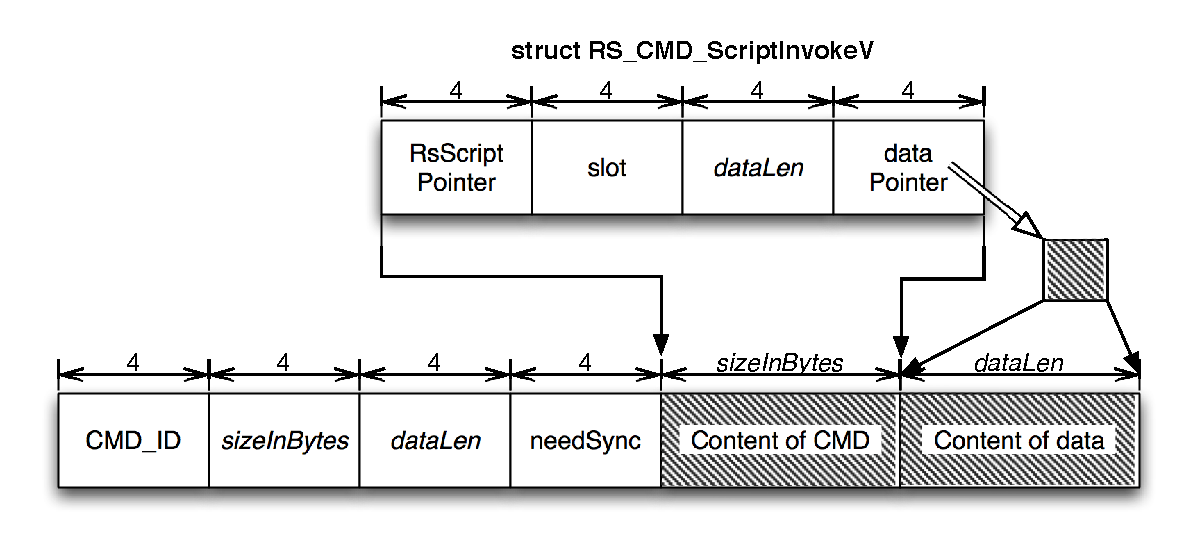
\includegraphics[scale=0.8]{fig/ScriptInvokeCMDEncoding.eps}
	\caption{RS\_CMD\_ScriptInvokeV encoding}
	\label{fig:ScriptInvokeCMDEncoding}
\end{center-figure}

\section{Transport Layer}
\label{s:rsListeningThread}
To receive commands, we choose socket to build \Transport{} for the the following reasons: (1) We need a lower-level implementation in \Core{}; (2) Bi-directional communication; and (3) Better performance of server side.

After the creation of RS context thread, we dynamically create the RS listening thread that depends on Android property. The following code shows our implementation.

\begin{lstlisting}
if (props.mRemoteServer) {
    pthread_t listeningThreadID;
    LOGV("create rsListeningThread");
    status = mIO.mToCore.receive(&listeningThreadID, &threadAttr, this);
    if (status) {
        LOGE("Failed to start rsListeningThread.");
        return false;
    }    
} else if (props.mRemoteClient){
    mIO.mToCore.initSocket();
} 
\end{lstlisting}

\paragraph{Server or Client?} The library of \RRS{} should support not only the client but also the server. A library for server and the other for client doesn't make sense if we want to accomplish the feature of two-way communication. For the reason, we stores the information through Android property system. For example, \RRS{} gets the property from \verb|props.mRemoteServer| and creates the RS listening thread if you type this in the ADB: 
\\\\ \verb|adb shell setprop remote.rs.server 1|\\\\

The idea of \RRS{} is straightforward, but it's still some issues we should take care. The following four subsection describes the challenge we encounter when extending \RS{} to \RRS{}.

\section{Replicated Command}
\label{s:rsListeningThread}
The key idea of \RRS{} is replaying the commands on the remote engine. Initially, any kind of \textit{commit()} and \textit{commitSync()} commands are followed by \textit{send()} and \textit{sendSync()} respectively.\footnote{Actually, we use sendCMD() instead of send() to avoid the confusion with socket send().} As a result, we found that it caused a error due to those replicated executed commands. For instance, binding the fragment twice might lead to chaos. The commands used for initialization should not be executed on the individual engine. In \Fountain{}, they are listed below in order:\\
\verb|RS_CMD_ID_ContextSetSurface|\\
\verb|RS_CMD_ID_ProgramFragmentCreate|\\
\verb|RS_CMD_ID_ContextBindProgramFragment|\\
\verb|RS_CMD_ID_ElementCreate|\\
\verb|RS_CMD_ID_ElementCreate2|\\
\verb|RS_CMD_ID_MeshCreate|\\
\verb|RS_CMD_ID_MeshBindIndex|\\
\verb|RS_CMD_ID_MeshBindVertex|\\
\verb|RS_CMD_ID_MeshInitVertexAttribs|\\
\verb|RS_CMD_ID_ScriptCCreate|\\
\verb|RS_CMD_ID_ScriptSetVarObj|\\
\verb|RS_CMD_ID_ScriptBindAllocation|\\
\verb|RS_CMD_ID_ContextBindRootScript|\\

\section{Command Synchornization}
\label{s:rsListeningThread}

As we mentioned in in prior chapter, a part of commands are put into the command queue via \textit{commitSync()}. That means \Client{} should be blocked until the command is flushed in \Core{}. Flushing in \RS{} refers to no command in the command queue. We demonstrate the design in Figure \ref{fig:LocklessFifo_pointer}. There are three markers in the figure:
\begin{itemize}
\item\textit{mGet} points to the memory address where the next command will be put.
\item\textit{mPut} points to the memory address where the next command will be popped.
\item\textit{mEnd} points to the memory address of end of the queue.
\end{itemize}
\begin{center-figure}
	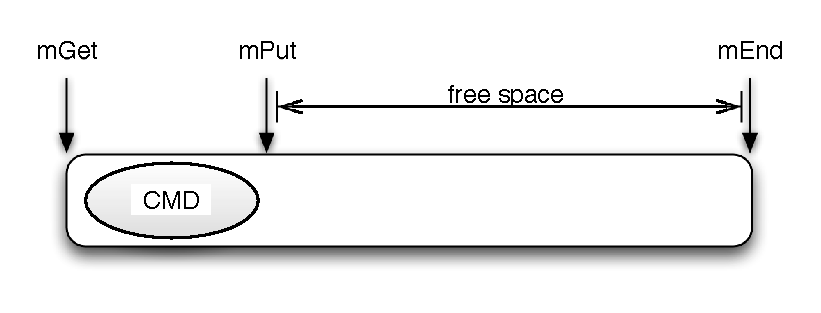
\includegraphics[scale=0.8]{fig/LocklessFifo_pointer.eps}
	\caption{Lockless FIFO command queue}
	\label{fig:LocklessFifo_pointer}
\end{center-figure}

Therefore, the command queue is flushed \textbf{if \textit{mGet} is equal to \textit{mPut}}.

Note that we have a \textit{sendSync()} for \RRS{}, the difference is the client (which sends the command) should be blocked instead of the server.

\section{Allocation of Command Queue}
\label{s:rsListeningThread}
Another stuff we should take care of the command queue is the allocation. In \RS{} implementation, either \textit{mToCore} or \textit{mToClient} are represented as a pointer and passed through functions by pointer. If we still pass the pointer to remote engine, it might cause a segamentation fault. As a result, we should remove it and get the correct \textit{mToCore} pointer.

\section{Handle the Pointer}
\label{s:rsListeningThread}
Like the allocation of command queue, almost variable are refered by pointer. So we should take care of it. For example, in \Fountain{}, we did that as the below:
\begin{lstlisting}
static inline void rsHCAPI_ScriptInvokeV (RsContext rsc, RsScript va, uint32_t slot, const void * data, uint32_t sizeBytes) {
    ThreadIO *io = &((Context *)rsc)->mIO;
    uint32_t size = sizeof(RS_CMD_ScriptInvokeV);
    if (sizeBytes < DATA_SYNC_SIZE) {
        size += (sizeBytes + 3) & ~3; 
    }   
    RS_CMD_ScriptInvokeV *cmd = static_cast<RS_CMD_ScriptInvokeV *>(io->mToCore.reserve(size));
    cmd->s = va; 
    cmd->slot = slot;
    cmd->dataLen = sizeBytes;
    cmd->data = data; 
    if (sizeBytes < DATA_SYNC_SIZE) {
        cmd->data = (void *)(cmd+1);
        memcpy(cmd+1, data, sizeBytes);
        io->mToCore.commit(RS_CMD_ID_ScriptInvokeV, size);
        if (&((Context *)rsc)->props.mRemoteClient)
            io->mToCore.sendCMD(RS_CMD_ID_ScriptInvokeV, size, cmd, cmd->dataLen, 0); 
    } else {
        io->mToCore.commitSync(RS_CMD_ID_ScriptInvokeV, size);
        io->mToCore.sendSync(RS_CMD_ID_ScriptInvokeV, size);
    }   

}
\end{lstlisting}


%1. 命令是會重複的, 不是所有的命令都需要傳送(有些是初始化動作)
%2. 有兩種命令,我們必須處理同步問題
%3. command queue 記憶體位址
%4. 有些命令的參數是包含指標的!






\chapter{Experiments}
\label{c:experiments}

The softwares selected in our experiments are all open-source software. A software may contains one or more executable programs. All programs are compiled to LLVM bitcodes using DragonEgg GCC plugin and LLVM toolchain as mentioned in \refchap{c:implementation} and the result bitcode is always optimized (\ie{} optimizer \verb|opt| with \verb|-O3| specified must have been performed on the result bitcode). Some of the programs contains single \verb|Makefile| and others use the GNU \verb|configure| and build system. In either case, most of the programs can be successfully compiled to bitcodes by modifying the rules in \verb|Makefile| without changing the source code. All experiments were performed on a dual CPU of Intel Xeon 2.33GHz 4-core processor machine and 2-GB of RAM running Gentoo Linux 2.6.31. Each core has only one processor (thread) and an 32-KB L1 data/instruction cache. Each pair of cores shares a 6-MB L2 on-chip cache.

\reftbl{t:exp-softwares} lists the size (lines of code), and the \textit{running time} when no any instrumentation codes are inserted for each programs. The programs are executed after using \JIT{} in \ThreadTracer{} to \textit{materialize} the bitcodes into host machine codes on-the-fly. The running time referred in our experiments only measured the time went into running the \verb|main| function. Besides, all timing measurements are the average of 10 runs.

\begin{center-table}
	\label{t:exp-softwares}
	\caption{List of the softwares examined in our experiments}
	\renewcommand{\arraystretch}{1.0}
	\begin{tabular}{| c | l | r | r | r | r |}
		\hline
		\multicolumn{1}{|c|}{\multirow{2}{*}{\textbf{Software}}} &
		\multicolumn{1}{c|}{\multirow{2}{*}{\textbf{Program}}} &
		\multicolumn{1}{c|}{\multirow{2}{2em}{\textbf{Size} (line)}} &
		\multicolumn{3}{c|}{\textbf{Base Time} (sec)} \\
		\cline{4-6}
		
		&
		&
		&
		\multicolumn{1}{c|}{\textbf{User}} &
		\multicolumn{1}{c|}{\textbf{System}} &
		\multicolumn{1}{c|}{\textbf{Total}}
		\\
		\hline\hline

		OpenMPagrep & % Software
		\texttt{agrep} & % Program
		\numprint{352} & % Size
		\numprint{18.31} & % User Time
		\numprint{2.25} & % System Time
		\numprint{20.56} % Total Time
		\\
		\hline\hline
		
		%HOMB & % Software
		%\texttt{homb} & % Program
		%\numprint{834} & % Size
		%\numprint{19.82} & % User Time
		%\numprint{0.13} & % System Time
		%\numprint{19.95} % Total Time
		%\\
		%\hline\hline

		%libsiftfast & % Software
		%\texttt{siftfast} & % Program
		%\numprint{2800} & % Size
		%\numprint{2.94} & % User Time
		%\numprint{0.051} & % System Time
		%\numprint{2.99} % Total Time
		%\\
		%\hline\hline

		\multirow{9}{*}{libgrid} & % Software
		\texttt{wf1d} & % Program
		\multirow{9}{*}{10661} & % Size
		\numprint{1.72} & % User Time
		\numprint{0.10} & % System Time
		\numprint{1.82} % Total Time
		\\

		& % Software
		\texttt{wf1d\_l} & % Program
		& % Size
		\numprint{0.06} & % User Time
		\numprint{0.002} & % System Time
		\numprint{0.06} % Total Time
		\\

		& % Software
		\texttt{wf1d\_nl} & % Program
		& % Size
		\numprint{0.08} & % User Time
		\numprint{0.006} & % System Time
		\numprint{0.08} % Total Time
		\\

		& % Software
		\texttt{wf2d} & % Program
		& % Size
		\numprint{2.22} & % User Time
		\numprint{0.004} & % System Time
		\numprint{2.23} % Total Time
		\\

		& % Software
		\texttt{wf2d\_l} & % Program
		& % Size
		\numprint{7.67} & % User Time
		\numprint{0.02} & % System Time
		\numprint{7.70} % Total Time
		\\

		& % Software
		\texttt{wf2d\_nl} & % Program
		& % Size
		\numprint{0.10} & % User Time
		\numprint{0.001} & % System Time
		\numprint{0.10} % Total Time
		\\
		
		& % Software
		\texttt{wf3d} & % Program
		& % Size
		\numprint{30.50} & % User Time
		\numprint{0.03} & % System Time
		\numprint{30.53} % Total Time
		\\

		& % Software
		\texttt{wf3d\_l} & % Program
		& % Size
		\numprint{23.84} & % User Time
		\numprint{0.01} & % System Time
		\numprint{23.85} % Total Time
		\\

		& % Software
		\texttt{wf3d\_nl} & % Program
		& % Size
		\numprint{2.48} & % User Time
		\numprint{0.004} & % System Time
		\numprint{2.49} % Total Time
		\\
		\hline\hline
		
		simple-ray-tracing & % Software
		\texttt{sray\_new\_load} & % Program
		\numprint{10460} & % Size
		\numprint{125.33} & % User Time
		\numprint{0.32} & % System Time
		\numprint{125.66} % Total Time
		\\
		\hline\hline
		
		\multirow{13}{*}{OmpSCR} & % Software
		\texttt{fft} & % Program
		\numprint{258} & % Size
		\numprint{0.64} & % User Time
		\numprint{0.04} & % System Time
		\numprint{0.68} % Total Time
		\\
		
		& % Software
		\texttt{fft6} & % Program
		\numprint{536} & % Size
		\numprint{0.078} & % User Time
		\numprint{0.001} & % System Time
		\numprint{0.08} % Total Time
		\\
		
		& % Software
		\texttt{testPath} & % Program
		\numprint{1730} & % Size
		\numprint{0.24} & % User Time
		\numprint{0.005} & % System Time
		\numprint{0.25} % Total Time
		\\
		
		& % Software
		\texttt{lu} & % Program
		\numprint{169} & % Size
		\numprint{0.15} & % User Time
		\numprint{0.001} & % System Time
		\numprint{0.15} % Total Time
		\\
		
		& % Software
		\texttt{md} & % Program
		\numprint{265} & % Size
		\numprint{0.18} & % User Time
		\numprint{0.002} & % System Time
		\numprint{0.18} % Total Time
		\\
		
		& % Software
		\texttt{pi} & % Program
		\numprint{83} & % Size
		\numprint{0.058} & % User Time
		\numprint{0} & % System Time
		\numprint{0.058} % Total Time
		\\
		
		& % Software
		\texttt{qsort} & % Program
		\numprint{168} & % Size
		\numprint{0.18} & % User Time
		\numprint{0.02} & % System Time
		\numprint{0.21} % Total Time
		\\
		
		& % Software
		\texttt{qsomp1} & % Program
		\numprint{345} & % Size
		\numprint{19.59} & % User Time
		\numprint{0.03} & % System Time
		\numprint{19.61} % Total Time
		\\
		
		& % Software
		\texttt{qsomp2} & % Program
		\numprint{387} & % Size
		\numprint{19.63} & % User Time
		\numprint{0.02} & % System Time
		\numprint{19.65} % Total Time
		\\
		
		& % Software
		\texttt{qsomp4} & % Program
		\numprint{405} & % Size
		\numprint{19.61} & % User Time
		\numprint{0.04} & % System Time
		\numprint{19.65} % Total Time
		\\
		
		& % Software
		\texttt{qsomp5} & % Program
		\numprint{302} & % Size
		\numprint{19.57} & % User Time
		\numprint{0.02} & % System Time
		\numprint{19.59} % Total Time
		\\
		
		& % Software
		\texttt{qsomp6} & % Program
		\numprint{411} & % Size
		\numprint{19.61} & % User Time
		\numprint{0.03} & % System Time
		\numprint{19.64} % Total Time
		\\
		\hline\hline
		
		Glucas & % Software
		\texttt{glucas} & % Program
		\numprint{51986} & % Size
		\numprint{1760.43} & % User Time
		\numprint{0.99} & % System Time
		\numprint{1761.42} % Total Time
		\\
		\hline
	\end{tabular}
\end{center-table}

We performed experiments on 24 programs listed above. The \texttt{agrep} is the implementation of \textsc{Agrep} algorithm~\cite{Wu:1991p1269} for approximate DNA string matching. The input set to \texttt{agrep} is the \textit{human genome} with 160 DNA sequence queries. The source code of \texttt{agrep} was modified to make it working under our Linux (it's originally for Windows only). The libgrid is a library for managing 1-D, 2-D and 3-D \textit{regular grids}. The programs containing in its package are to propagate the Schr\"odinger equation~\cite{Schrodinger:1926p1292} linearly and non-linearly in a 1-D, 2-D and 3-D regular grid. The OmpSCR, abbreviated from OpenMP Source Code Repository, contains several small programs written using OpenMP directives. The \texttt{fft}, a Cooley-Tukey fast Fourier transform (FFT) algorithm~\cite{Cooley:1965p1293} implementation; the \texttt{fft6}, a Bailey's 6-step 1D FFT method implementation~\cite{Bailey:1989p1295}; the \texttt{testPath}, test whether there exists a path between given two nodes in a directed graph; the \texttt{lu}, LU decomposition of a 2-D matrix; \texttt{md}, a simple molecular dynamics simulation~\cite{Swope:1982p1298}; the \texttt{pi}, calculation of $\pi$ values; the \texttt{qsort}, C implementation of Quicksort algorithm~\cite{Hoare:1962p1297} for integer array; the \texttt{qsomp1}, \texttt{qsomp2}, \dots, and \texttt{qsomp6}, each is a variation of Quicksort algorithm implemented in C++; the \texttt{glucas}, primality test for Mersenne numbers. All the programs are \textit{compute-bound}.

%%%%%%%%%%%%%%%%%%%%%%%%%%%%%%%%%%%%%%%%%%%%%%%%%%%%%%%%%%%%%%%%%%%%
\section{Evaluation of Dynamic Data Race Detector}
\begin{center-table}
	\label{t:exp-results-no-omptsa}
	\caption{Experiment results (static data race detector excluded) }
	\renewcommand{\arraystretch}{1.0}
	\begin{tabular}{| l | r | r |  r | r | c | r | c |}
		\hline
		\multicolumn{1}{|c|}{\textbf{Program}} &
		\multicolumn{1}{|c}{\begin{sideways}\textbf{\# instrumentation inserted}\end{sideways}} &
		\multicolumn{1}{|c}{\begin{sideways}\textbf{\# active instrumentation}\end{sideways}} &
		\multicolumn{1}{|c}{\begin{sideways}\textbf{\# \texttt{TTVar}s created}\end{sideways}} &
		\multicolumn{1}{|c}{\begin{sideways}\textbf{\# \texttt{onVarAccess} events}\end{sideways}} &
		\multicolumn{1}{|c}{\begin{sideways}\textbf{Percentage of array access}\end{sideways}} &
		\multicolumn{1}{|c}{\begin{sideways}\textbf{Slowdown} (x Base Time)\end{sideways}} &
		\multicolumn{1}{|c|}{\begin{sideways}\textbf{\# Data races found}\end{sideways}}
		\\
		\hline\hline
		
		\texttt{agrep} & % Program
		\numprint{48} & % # instrumentation codes
		\numprint{2} & % # active instrumentation
		\numprint{1} & % # TTVars created
		\numprint{10368} & % # onVarAccess events
		\numprint{0}~\% & % Percentage of array access
		\numprint{0.01} & % Slowdown
		\numprint{0} % # Data races found
		\\
		
		\texttt{wf1d} & % Program
		\numprint{1647} & % # instrumentation codes
		\numprint{73} & % # active instrumentation
		\numprint{20051} & % # TTVars created
		\numprint{32}~M & % # onVarAccess events
		\numprint{56.19}~\% & % Percentage of array access
		\numprint{4.27} & % Slowdown
		\numprint{0} % # Data races found
		\\
		
		\texttt{wf1d\_l} & % Program
		\numprint{1647} & % # instrumentation codes
		\numprint{134} & % # active instrumentation
		\numprint{1506} & % # TTVars created
		\numprint{3227}~K & % # onVarAccess events
		\numprint{60.58}~\% & % Percentage of array access
		\numprint{13.4} & % Slowdown
		\numprint{0} % # Data races found
		\\
		
		\texttt{wf1d\_nl} & % Program
		\numprint{1647} & % # instrumentation codes
		\numprint{119} & % # active instrumentation
		\numprint{12217} & % # TTVars created
		\numprint{4408}~K & % # onVarAccess events
		\numprint{49.24}~\% & % Percentage of array access
		\numprint{14.32} & % Slowdown
		\numprint{0} % # Data races found
		\\
		
		\texttt{wf2d} & % Program
		\numprint{1647} & % # instrumentation codes
		\numprint{99} & % # active instrumentation
		\numprint{65608} & % # TTVars created
		\numprint{137}~M & % # onVarAccess events
		\numprint{57.06}~\% & % Percentage of array access
		\numprint{17.05} & % Slowdown
		\numprint{0} % # Data races found
		\\
		
		\texttt{wf2d\_l} & % Program
		\numprint{1647} & % # instrumentation codes
		\numprint{164} & % # active instrumentation
		\numprint{19889} & % # TTVars created
		\numprint{783}~M & % # onVarAccess events
		\numprint{64.97}~\% & % Percentage of array access
		\numprint{25.14} & % Slowdown
		\numprint{0} % # Data races found
		\\
		
		\texttt{wf2d\_nl} & % Program
		\numprint{1647} & % # instrumentation codes
		\numprint{138} & % # active instrumentation
		\numprint{11163} & % # TTVars created
		\numprint{6410}~K & % # onVarAccess events
		\numprint{52.76}~\% & % Percentage of array access
		\numprint{10.70} & % Slowdown
		\numprint{0} % # Data races found
		\\
	
		\texttt{wf3d} & % Program
		\numprint{1647} & % # instrumentation codes
		\numprint{118} & % # active instrumentation
		\numprint{1310}~K & % # TTVars created
		\numprint{1698}~M & % # onVarAccess events
		\numprint{98.83}~\% & % Percentage of array access
		\numprint{68.07} & % Slowdown
		\numprint{0} % # Data races found
		\\
		
		\texttt{wf3d\_l} & % Program
		\numprint{1647} & % # instrumentation codes
		\numprint{190} & % # active instrumentation
		\numprint{460}~K & % # TTVars created
		\numprint{273}~M & % # onVarAccess events
		\numprint{92.86}~\% & % Percentage of array access
		\numprint{39.19} & % Slowdown
		\numprint{0} % # Data races found
		\\
		
		\texttt{wf3d\_nl} & % Program
		\numprint{1647} & % # instrumentation codes
		\numprint{162} & % # active instrumentation
		\numprint{491}~K & % # TTVars created
		\numprint{165}~M & % # onVarAccess events
		\numprint{97.32}~\% & % Percentage of array access
		\numprint{69.52} & % Slowdown
		\numprint{0} % # Data races found
		\\
		
		\texttt{sray\_new\_load} & % Program
		\numprint{1} & % # instrumentation codes
		\numprint{1} & % # active instrumentation
		\numprint{1} & % # TTVars created
		\numprint{7} & % # onVarAccess events
		\numprint{0}~\% & % Percentage of array access
		\numprint{0.16} & % Slowdown
		\numprint{0} % # Data races found
		\\
		
		\texttt{fft} & % Program
		\numprint{32} & % # instrumentation codes
		\numprint{0} & % # active instrumentation
		\numprint{328}~K & % # TTVars created
		\numprint{13}~M & % # onVarAccess events
		\numprint{29.58}~\% & % Percentage of array access
		\numprint{119.10} & % Slowdown
		\numprint{0} % # Data races found
		\\
		
		\texttt{fft6} & % Program
		\numprint{94} & % # instrumentation codes
		\numprint{94} & % # active instrumentation
		\numprint{90250} & % # TTVars created
		\numprint{1247}~K & % # onVarAccess events
		\numprint{66.28}~\% & % Percentage of array access
		\numprint{158.97} & % Slowdown
		\numprint{0} % # Data races found
		\\
		
		\texttt{testPath} & % Program
		\numprint{32} & % # instrumentation codes
		\numprint{30} & % # active instrumentation
		\numprint{25729} & % # TTVars created
		\numprint{78615} & % # onVarAccess events
		\numprint{22.11}~\% & % Percentage of array access
		\numprint{14.45} & % Slowdown
		\numprint{13} % # Data races found
		\\
		
		\texttt{lu} & % Program
		\numprint{24} & % # instrumentation codes
		\numprint{24} & % # active instrumentation
		\numprint{60304} & % # TTVars created
		\numprint{29}~M & % # onVarAccess events
		\numprint{63.33}~\% & % Percentage of array access
		\numprint{2019.73} & % Slowdown
		\numprint{0} % # Data races found
		\\
		
		\texttt{md} & % Program
		\numprint{52} & % # instrumentation codes
		\numprint{48} & % # active instrumentation
		\numprint{6189} & % # TTVars created
		\numprint{78}~M & % # onVarAccess events
		\numprint{44.40}~\% & % Percentage of array access
		\numprint{4374.74} & % Slowdown
		\numprint{0} % # Data races found
		\\
		
		\texttt{pi} & % Program
		\numprint{3} & % # instrumentation codes
		\numprint{3} & % # active instrumentation
		\numprint{3} & % # TTVars created
		\numprint{26.4} & % # onVarAccess events
		\numprint{0}~\% & % Percentage of array access
		\numprint{0.34} & % Slowdown
		\numprint{0} % # Data races found
		\\
		
		\texttt{qsort} & % Program
		\numprint{5} & % # instrumentation codes
		\numprint{0} & % # active instrumentation
		\numprint{7} & % # TTVars created
		\numprint{50} & % # onVarAccess events
		\numprint{40}~\% & % Percentage of array access
		\numprint{1.21} & % Slowdown
		\numprint{0} % # Data races found
		\\
		
		\texttt{qsomp1} & % Program
		\numprint{13} & % # instrumentation codes
		\numprint{7} & % # active instrumentation
		\numprint{6} & % # TTVars created
		\numprint{7} & % # onVarAccess events
		\numprint{0}~\% & % Percentage of array access
		\numprint{0.00} & % Slowdown
		\numprint{0} % # Data races found
		\\
		
		\texttt{qsomp2} & % Program
		\numprint{17} & % # instrumentation codes
		\numprint{9} & % # active instrumentation
		\numprint{8} & % # TTVars created
		\numprint{9} & % # onVarAccess events
		\numprint{0}~\% & % Percentage of array access
		\numprint{0.00} & % Slowdown
		\numprint{0} % # Data races found
		\\
		
		\texttt{qsomp4} & % Program
		\numprint{17} & % # instrumentation codes
		\numprint{9} & % # active instrumentation
		\numprint{8} & % # TTVars created
		\numprint{9} & % # onVarAccess events
		\numprint{0}~\% & % Percentage of array access
		\numprint{0.00} & % Slowdown
		\numprint{0} % # Data races found
		\\
		
		\texttt{qsomp5} & % Program
		\numprint{10} & % # instrumentation codes
		\numprint{0} & % # active instrumentation
		\numprint{0} & % # TTVars created
		\numprint{0} & % # onVarAccess events
		\numprint{0}~\% & % Percentage of array access
		\numprint{0.00} & % Slowdown
		\numprint{0} % # Data races found
		\\
		
		\texttt{qsomp6} & % Program
		\numprint{17} & % # instrumentation codes
		\numprint{9} & % # active instrumentation
		\numprint{8} & % # TTVars created
		\numprint{9} & % # onVarAccess events
		\numprint{0}~\% & % Percentage of array access
		\numprint{0.00} & % Slowdown
		\numprint{0} % # Data races found
		\\
		
		\texttt{glucas} & % Program
		\numprint{122} & % # instrumentation codes
		\numprint{120} & % # active instrumentation
		\numprint{65} & % # TTVars created
		\numprint{593}~K & % # onVarAccess events
		\numprint{17.09}~\% & % Percentage of array access
		\numprint{0.01} & % Slowdown
		\numprint{1} % # Data races found
		\\
		\hline
	\end{tabular}
\end{center-table}

The results of experiments performed without help from static data race detector are shown in \reftbl{t:exp-results-no-omptsa}. The first column lists the number of instrumentation codes inserted by \Rewriter{} which is equal to the number of \verb|load| and \verb|store| instructions instrumented. The second column is the number of \textit{active instrumentation} which is the actual instrumentation used at runtime. Then the number of shadow variables (\ie{} \verb|TTVar| instances) created during the execution and the times \verb|VarAccess| events triggered are listed in column 3 and 4, respectively. We also show the percentage of array access in the \verb|VarAccess| events. Large numbers are chopped off with K and M denoting a multiple of one thousand and one million, respectively. The data races detected in our experiments are all confirmed to be \textit{true} data races. And some of them are \textit{harmful data races}~\cite{Narayanasamy:2007p819} (\ie{} data races found in \texttt{testPath}). Once there's any data race detected in a program, we manually fixed it and re-run all experiments for that program.

In general, our dynamic data race detector incurs overheads spanning from $1x$ to $160x$ approximately. The programs above incurred significant runtime overheads have one thing in common --- their memory access pattern are \textit{complicated} or even \textit{random}. For example, the \texttt{md} has an array access in the nested loop with depth 5 and complex array element accessing. The \texttt{fft} uses the divide and conquer strategy and \textit{recursive call} in FFT implementation which also hurts the locality. Other programs like \texttt{wf3d} and \texttt{wf3d\_l}, though they generated lots of \verb|VarAccess| events several times than \verb|lu|,  \verb|md|, \etc{} and full of the array element accesses, they have good access patterns which allocate and access the 3-D grid data structure \textit{in sequential order}. One can also reach the same conclusion by comparing \texttt{testPath} and \texttt{wf1d}. Obviously, \texttt{wf1d} generates much more \verb|VarAccess| events in a roughly $408x$ and more array access percentage in a roughly $3x$ while the slowdown incurred by \texttt{wf1d} is three times less than \texttt{testPath}. That is because \texttt{testPath} uses \textit{adjacency list} to represent the graph resulting the unstructured memory access pattern during the graph traversal (two adjacent nodes may be far away from each other in the memory). 

%%%%%%%%%%%%%%%%%%%%%%%%%%%%%%%%%%%%%%%%%%%%%%%%%%%%%%%%%%%%%%%%%%%%

\section{Evaluation of Dynamic Data Race Detector with Static Approach}
\begin{center-table}
	\label{t:exp-results-omptsa}
	\caption{Experiment results (static data race detector included) }
	\renewcommand{\arraystretch}{1.0}
	\begin{tabular}{| l | r | r |  r | r | c | r | c |}
		\hline
		\multicolumn{1}{|c|}{\textbf{Program}} &
		\multicolumn{1}{|c}{\begin{sideways}\textbf{\# instrumentation inserted}\end{sideways}} &
		\multicolumn{1}{|c}{\begin{sideways}\textbf{\# active instrumentation}\end{sideways}} &
		\multicolumn{1}{|c}{\begin{sideways}\textbf{\# \texttt{TTVar}s created}\end{sideways}} &
		\multicolumn{1}{|c}{\begin{sideways}\textbf{\# \texttt{onVarAccess} events}\end{sideways}} &
		\multicolumn{1}{|c}{\begin{sideways}\textbf{Percentage of array access}\end{sideways}} &
		\multicolumn{1}{|c}{\begin{sideways}\textbf{Slowdown} (x Base Time)\end{sideways}} &
		\multicolumn{1}{|c}{\begin{sideways}\textbf{Performance improvement}\end{sideways}}
		\\
		\hline\hline
		
		\texttt{agrep} & % Program
		\numprint{48} & % # instrumentation codes
		\numprint{2} & % # active instrumentation
		\numprint{1} & % # TTVars created
		\numprint{10368} & % # onVarAccess events
		\numprint{0}~\% & % Percentage of array access
		\numprint{0.01} & % Slowdown
		\numprint{0} % Performance improvement
		\\
		
		\texttt{wf1d} & % Program
		\numprint{1423} & % # instrumentation codes
		\numprint{73} & % # active instrumentation
		\numprint{20051} & % # TTVars created
		\numprint{32}~M & % # onVarAccess events
		\numprint{56.19}~\% & % Percentage of array access
		\numprint{4.27} & % Slowdown
		\numprint{0} % Performance improvement
		\\
		
		\texttt{wf1d\_l} & % Program
		\numprint{1487} & % # instrumentation codes
		\numprint{125} & % # active instrumentation
		\numprint{1417} & % # TTVars created
		\numprint{3226}~K & % # onVarAccess events
		\numprint{70.78}~\% & % Percentage of array access
		\numprint{12.35} & % Slowdown
		\numprint{1.05} % Performance improvement
		\\
		
		\texttt{wf1d\_nl} & % Program
		\numprint{1423} & % # instrumentation codes
		\numprint{103} & % # active instrumentation
		\numprint{12158} & % # TTVars created
		\numprint{4308}~K & % # onVarAccess events
		\numprint{54.75}~\% & % Percentage of array access
		\numprint{14.32} & % Slowdown
		\numprint{1.3} % Performance improvement
		\\
		
		\texttt{wf2d} & % Program
		\numprint{1423} & % # instrumentation codes
		\numprint{77} & % # active instrumentation
		\numprint{65321} & % # TTVars created
		\numprint{137}~M & % # onVarAccess events
		\numprint{58.69}~\% & % Percentage of array access
		\numprint{15.35} & % Slowdown
		\numprint{1.7} % Performance improvement
		\\
		
		\texttt{wf2d\_l} & % Program
		\numprint{1423} & % # instrumentation codes
		\numprint{135} & % # active instrumentation
		\numprint{19729} & % # TTVars created
		\numprint{783}~M & % # onVarAccess events
		\numprint{69.5}~\% & % Percentage of array access
		\numprint{23.42} & % Slowdown
		\numprint{1.72} % Performance improvement
		\\
		
		\texttt{wf2d\_nl} & % Program
		\numprint{1423} & % # instrumentation codes
		\numprint{116} & % # active instrumentation
		\numprint{11132} & % # TTVars created
		\numprint{6410}~K & % # onVarAccess events
		\numprint{52.76}~\% & % Percentage of array access
		\numprint{10.70} & % Slowdown
		\numprint{0} % Performance improvement
		\\
	
		\texttt{wf3d} & % Program
		\numprint{1423} & % # instrumentation codes
		\numprint{118} & % # active instrumentation
		\numprint{1310}~K & % # TTVars created
		\numprint{1698}~M & % # onVarAccess events
		\numprint{98.83}~\% & % Percentage of array access
		\numprint{68.07} & % Slowdown
		\numprint{0} % Performance improvement
		\\
		
		\texttt{wf3d\_l} & % Program
		\numprint{1423} & % # instrumentation codes
		\numprint{190} & % # active instrumentation
		\numprint{460}~K & % # TTVars created
		\numprint{273}~M & % # onVarAccess events
		\numprint{92.86}~\% & % Percentage of array access
		\numprint{39.19} & % Slowdown
		\numprint{0} % Performance improvement
		\\
		
		\texttt{wf3d\_nl} & % Program
		\numprint{1423} & % # instrumentation codes
		\numprint{162} & % # active instrumentation
		\numprint{491}~K & % # TTVars created
		\numprint{165}~M & % # onVarAccess events
		\numprint{97.32}~\% & % Percentage of array access
		\numprint{69.52} & % Slowdown
		\numprint{0} % Performance improvement
		\\
		
		\texttt{sray\_new\_load} & % Program
		\numprint{1} & % # instrumentation codes
		\numprint{1} & % # active instrumentation
		\numprint{1} & % # TTVars created
		\numprint{7} & % # onVarAccess events
		\numprint{0}~\% & % Percentage of array access
		\numprint{0.16} & % Slowdown
		\numprint{0} % Performance improvement
		\\
		
		\texttt{fft} & % Program
		\numprint{27} & % # instrumentation codes
		\numprint{27} & % # active instrumentation
		\numprint{328}~K & % # TTVars created
		\numprint{13}~M & % # onVarAccess events
		\numprint{30.68}~\% & % Percentage of array access
		\numprint{119.07} & % Slowdown
		\numprint{0.03} % Performance improvement
		\\
		
		\texttt{fft6} & % Program
		\numprint{87} & % # instrumentation codes
		\numprint{87} & % # active instrumentation
		\numprint{90245} & % # TTVars created
		\numprint{1226}~K & % # onVarAccess events
		\numprint{69.72}~\% & % Percentage of array access
		\numprint{157.89} & % Slowdown
		\numprint{1.08} % Performance improvement
		\\
		
		\texttt{testPath} & % Program
		\numprint{32} & % # instrumentation codes
		\numprint{30} & % # active instrumentation
		\numprint{25729} & % # TTVars created
		\numprint{78615} & % # onVarAccess events
		\numprint{22.11}~\% & % Percentage of array access
		\numprint{14.45} & % Slowdown
		\numprint{13} % Performance improvement
		\\
		
		\texttt{lu} & % Program
		\numprint{20} & % # instrumentation codes
		\numprint{20} & % # active instrumentation
		\numprint{60256} & % # TTVars created
		\numprint{29}~M & % # onVarAccess events
		\numprint{67.54}~\% & % Percentage of array access
		\numprint{2018.66} & % Slowdown
		\numprint{1.07} % Performance improvement
		\\
		
		\texttt{md} & % Program
		\numprint{48} & % # instrumentation codes
		\numprint{44} & % # active instrumentation
		\numprint{6176} & % # TTVars created
		\numprint{78}~M & % # onVarAccess events
		\numprint{47.39}~\% & % Percentage of array access
		\numprint{4373.28} & % Slowdown
		\numprint{1.46} % Performance improvement
		\\
		
		\texttt{pi} & % Program
		\numprint{3} & % # instrumentation codes
		\numprint{3} & % # active instrumentation
		\numprint{3} & % # TTVars created
		\numprint{26.4} & % # onVarAccess events
		\numprint{0}~\% & % Percentage of array access
		\numprint{0.34} & % Slowdown
		\numprint{0} % Performance improvement
		\\
		
		\texttt{qsort} & % Program
		\numprint{5} & % # instrumentation codes
		\numprint{5} & % # active instrumentation
		\numprint{7} & % # TTVars created
		\numprint{50} & % # onVarAccess events
		\numprint{40}~\% & % Percentage of array access
		\numprint{1.21} & % Slowdown
		\numprint{0} % Performance improvement
		\\
		
		\texttt{qsomp1} & % Program
		\numprint{13} & % # instrumentation codes
		\numprint{7} & % # active instrumentation
		\numprint{6} & % # TTVars created
		\numprint{7} & % # onVarAccess events
		\numprint{0}~\% & % Percentage of array access
		\numprint{0.00} & % Slowdown
		\numprint{0} % Performance improvement
		\\
		
		\texttt{qsomp2} & % Program
		\numprint{17} & % # instrumentation codes
		\numprint{9} & % # active instrumentation
		\numprint{8} & % # TTVars created
		\numprint{9} & % # onVarAccess events
		\numprint{0}~\% & % Percentage of array access
		\numprint{0.00} & % Slowdown
		\numprint{0} % Performance improvement
		\\
		
		\texttt{qsomp4} & % Program
		\numprint{17} & % # instrumentation codes
		\numprint{9} & % # active instrumentation
		\numprint{8} & % # TTVars created
		\numprint{9} & % # onVarAccess events
		\numprint{0}~\% & % Percentage of array access
		\numprint{0.00} & % Slowdown
		\numprint{0} % Performance improvement
		\\
		
		\texttt{qsomp5} & % Program
		\numprint{10} & % # instrumentation codes
		\numprint{0} & % # active instrumentation
		\numprint{0} & % # TTVars created
		\numprint{0} & % # onVarAccess events
		\numprint{0}~\% & % Percentage of array access
		\numprint{0.00} & % Slowdown
		\numprint{0} % Performance improvement
		\\
		
		\texttt{qsomp6} & % Program
		\numprint{17} & % # instrumentation codes
		\numprint{9} & % # active instrumentation
		\numprint{8} & % # TTVars created
		\numprint{9} & % # onVarAccess events
		\numprint{0}~\% & % Percentage of array access
		\numprint{0.00} & % Slowdown
		\numprint{0} % Performance improvement
		\\
		
		\texttt{glucas} & % Program
		\numprint{111} & % # instrumentation codes
		\numprint{109} & % # active instrumentation
		\numprint{54} & % # TTVars created
		\numprint{593}~K & % # onVarAccess events
		\numprint{20.23}~\% & % Percentage of array access
		\numprint{0.00} & % Slowdown
		\numprint{0.01} % Performance improvement
		\\
		\hline
	\end{tabular}
\end{center-table}

\reftbl{t:exp-results-omptsa} shows the evaluation which combine our static detector with the dynamic detector. The performance improvement column is defined by the difference between slowdown excluding (in \reftbl{t:exp-results-no-omptsa}) and including the static data race detector. Our static data race detector doesn't improve the performance significantly. The main reason is that our static data race detector makes oversimplified assumption on the array accesses in the program --- they are aliased and always induced the data races. Therefore, our static detector is unable to eliminate any array access instrumentation which is the real bottleneck of the performance. The set of the data races found in the previous experiment remains unchanged after the static data race detector is included. Later experiments use the execution time from the configuration in this experiments as the base time.

%%%%%%%%%%%%%%%%%%%%%%%%%%%%%%%%%%%%%%%%%%%%%%%%%%%%%%%%%%%%%%%%%%%%
\section{Evaluation of Real-to-Shadow Map Lookup Cache}
\begin{center-table}
  \label{t:exp-results-real-to-shadow-variable-cache}
  \caption[Real-to-shadow variable map lookup cache comparison]{Comparison between real-to-shadow variable map lookup cache in \ThreadTracer{} and \RoadRunner{}}
  \renewcommand{\arraystretch}{1.0}
  \begin{tabular}{| l | r | r | r | r | r | c |}
    \hline
	&
    &
    \multicolumn{2}{c|}{\textbf{\ThreadTracer{}}} &
    \multicolumn{2}{c|}{\textbf{\RoadRunner{}}} &
	\\
    \cline{3-6}
    
    \multicolumn{1}{|c|}{\textbf{Program}} &
    \multicolumn{1}{c|}{\begin{sideways}\textbf{\# hit in thread-local cache}\end{sideways}} &
    \multicolumn{1}{c}{\begin{sideways}\textbf{\# hit in thread-shared cache}\end{sideways}} &
    \multicolumn{1}{|c}{\textbf{Hit Rate}} &
    \multicolumn{1}{|c}{\begin{sideways}\textbf{\# hit in thread-shared cache}\end{sideways}} &
    \multicolumn{1}{|c|}{\textbf{Hit Rate}} &
	\multicolumn{1}{c|}{\begin{sideways}\textbf{Effectiveness}\end{sideways}}
    \\
    \hline\hline
    
    \texttt{agrep} & % Program
    \numprint{10304} & % # hit in thread-local cache
    \numprint{63} & % # hit in thread-shared cach
    \numprint{99.99}~\% & % Hit Rate
    \numprint{63} & % # hit in thread-shared cache
    \numprint{99.99}~\% & % Hit Rate
    \numprint{1.001} % Effectiveness
    \\
    
    \texttt{wf1d} & % Program
    \numprint{32}~M & % # hit in thread-local cache
    \numprint{5373} & % # hit in thread-shared cach
    \numprint{99.99}~\% & % Hit Rate
    \numprint{9367} & % # hit in thread-shared cache
    \numprint{99.99}~\% & % Hit Rate
    \numprint{1.007} % Effectiveness
    \\
    
    \texttt{wf1d\_l} & % Program
    \numprint{3095}~K & % # hit in thread-local cache
    \numprint{72714} & % # hit in thread-shared cach
    \numprint{98.17}~\% & % Hit Rate
    \numprint{131}~K & % # hit in thread-shared cache
    \numprint{99.99}~\% & % Hit Rate
    \numprint{1.007} % Effectiveness
    \\
    
    \texttt{wf1d\_nl} & % Program
    \numprint{4238}~K & % # hit in thread-local cache
    \numprint{91563} & % # hit in thread-shared cach
    \numprint{98.22}~\% & % Hit Rate
    \numprint{169}~K & % # hit in thread-shared cache
    \numprint{99.99}~\% & % Hit Rate
    \numprint{1.011} % Effectiveness
    \\
    
    \texttt{wf2d} & % Program
    \numprint{137}~M & % # hit in thread-local cache
    \numprint{7762} & % # hit in thread-shared cach
    \numprint{99.99}~\% & % Hit Rate
    \numprint{14951} & % # hit in thread-shared cache
    \numprint{99.99}~\% & % Hit Rate
    \numprint{0.997} % Effectiveness
    \\
    
    \texttt{wf2d\_l} & % Program
    \numprint{766}~M & % # hit in thread-local cache
    \numprint{6632}~K & % # hit in thread-shared cach
    \numprint{98.67}~\% & % Hit Rate
    \numprint{17}~M & % # hit in thread-shared cache
    \numprint{99.99}~\% & % Hit Rate
    \numprint{0.997} % Effectiveness
    \\
    
    \texttt{wf2d\_nl} & % Program
    \numprint{6399}~K & % # hit in thread-local cache
    \numprint{5803} & % # hit in thread-shared cach
    \numprint{99.93}~\% & % Hit Rate
    \numprint{10293} & % # hit in thread-shared cache
    \numprint{99.99}~\% & % Hit Rate
    \numprint{1.000} % Effectiveness
    \\
  
    \texttt{wf3d} & % Program
    \numprint{1698}~M & % # hit in thread-local cache
    \numprint{1796} & % # hit in thread-shared cach
    \numprint{99.998}~\% & % Hit Rate
    \numprint{22134} & % # hit in thread-shared cache
    \numprint{99.99}~\% & % Hit Rate
    \numprint{1.008} % Effectiveness
    \\
    
    \texttt{wf3d\_l} & % Program
    \numprint{2731}~M & % # hit in thread-local cache
    \numprint{7499} & % # hit in thread-shared cach
    \numprint{99.90}~\% & % Hit Rate
    \numprint{2717}~K & % # hit in thread-shared cache
    \numprint{99.99}~\% & % Hit Rate
    \numprint{1.006} % Effectiveness
    \\
    
    \texttt{wf3d\_nl} & % Program
    \numprint{165}~M & % # hit in thread-local cache
    \numprint{1867} & % # hit in thread-shared cach
    \numprint{99.99}~\% & % Hit Rate
    \numprint{18278} & % # hit in thread-shared cache
    \numprint{99.99}~\% & % Hit Rate
    \numprint{0.999} % Effectiveness
    \\
    
    \texttt{sray\_new\_load} & % Program
    \numprint{0} & % # hit in thread-local cache
    \numprint{5.4} & % # hit in thread-shared cach
    \numprint{77.14}~\% & % Hit Rate
    \numprint{6} & % # hit in thread-shared cache
    \numprint{85.71}~\% & % Hit Rate
    \numprint{1.002} % Effectiveness
    \\
    
    \texttt{fft} & % Program
    \numprint{7634}~K & % # hit in thread-local cache
    \numprint{1592}~K & % # hit in thread-shared cach
    \numprint{66.10}~\% & % Hit Rate
    \numprint{4699}~K & % # hit in thread-shared cache
    \numprint{88.36}~\% & % Hit Rate
    \numprint{1.164} % Effectiveness
    \\
    
    \texttt{fft6} & % Program
    \numprint{1205}~K & % # hit in thread-local cache
    \numprint{338.6} & % # hit in thread-shared cach
    \numprint{96.69}~\% & % Hit Rate
    \numprint{337} & % # hit in thread-shared cache
    \numprint{84.60}~\% & % Hit Rate
    \numprint{1.011} % Effectiveness
    \\
    
    \texttt{testPath} & % Program
    \numprint{63695} & % # hit in thread-local cache
    \numprint{38291} & % # hit in thread-shared cach
    \numprint{77.96}~\% & % Hit Rate
    \numprint{49710} & % # hit in thread-shared cache
    \numprint{77.98}~\% & % Hit Rate
    \numprint{1.010} % Effectiveness
    \\
    
    \texttt{lu} & % Program
    \numprint{10}~M & % # hit in thread-local cache
    \numprint{16}~M & % # hit in thread-shared cach
    \numprint{91.33}~\% & % Hit Rate
    \numprint{18}~M & % # hit in thread-shared cache
    \numprint{99.88}~\% & % Hit Rate
    \numprint{0.977} % Effectiveness
    \\
    
    \texttt{md} & % Program
    \numprint{75}~M & % # hit in thread-local cache
    \numprint{113}~K & % # hit in thread-shared cach
    \numprint{96.25}~\% & % Hit Rate
    \numprint{1847}~K & % # hit in thread-shared cache
    \numprint{98.47}~\% & % Hit Rate
    \numprint{0.990} % Effectiveness
    \\
    
    \texttt{pi} & % Program
    \numprint{0} & % # hit in thread-local cache
    \numprint{21} & % # hit in thread-shared cach
    \numprint{79.55}~\% & % Hit Rate
    \numprint{21} & % # hit in thread-shared cache
    \numprint{79.55}~\% & % Hit Rate
    \numprint{1.001} % Effectiveness
    \\
    
    \texttt{qsort} & % Program
    \numprint{45} & % # hit in thread-local cache
    \numprint{0} & % # hit in thread-shared cach
    \numprint{90.00}~\% & % Hit Rate
    \numprint{0} & % # hit in thread-shared cache
    \numprint{90.00}~\% & % Hit Rate
    \numprint{1.002} % Effectiveness
    \\
    
    \texttt{qsomp1} & % Program
    \numprint{1} & % # hit in thread-local cache
    \numprint{0} & % # hit in thread-shared cach
    \numprint{14.29}~\% & % Hit Rate
    \numprint{0} & % # hit in thread-shared cache
    \numprint{14.29}~\% & % Hit Rate
    \numprint{1.000} % Effectiveness
    \\
    
    \texttt{qsomp2} & % Program
    \numprint{1} & % # hit in thread-local cache
    \numprint{0} & % # hit in thread-shared cach
    \numprint{11.11}~\% & % Hit Rate
    \numprint{0} & % # hit in thread-shared cache
    \numprint{11.11}~\% & % Hit Rate
    \numprint{1.000} % Effectiveness
    \\
    
    \texttt{qsomp4} & % Program
    \numprint{1} & % # hit in thread-local cache
    \numprint{0} & % # hit in thread-shared cach
    \numprint{11.11}~\% & % Hit Rate
    \numprint{0} & % # hit in thread-shared cache
    \numprint{11.11}~\% & % Hit Rate
    \numprint{1.000} % Effectiveness
    \\
    
    \texttt{qsomp5} & % Program
    \numprint{0} & % # hit in thread-local cache
    \numprint{0} & % # hit in thread-shared cach
    \numprint{0}~\% & % Hit Rate
    \numprint{0} & % # hit in thread-shared cache
    \numprint{0}~\% & % Hit Rate
    \numprint{1.000} % Effectiveness
    \\
    
    \texttt{qsomp6} & % Program
    \numprint{1} & % # hit in thread-local cache
    \numprint{0} & % # hit in thread-shared cach
    \numprint{11.11}~\% & % Hit Rate
    \numprint{0} & % # hit in thread-shared cache
    \numprint{11.11}~\% & % Hit Rate
    \numprint{1.000} % Effectiveness
    \\
    
    \texttt{glucas} & % Program
    \numprint{61615} & % # hit in thread-local cache
    \numprint{531}~K & % # hit in thread-shared cach
    \numprint{99.89}~\% & % Hit Rate
    \numprint{523}~K & % # hit in thread-shared cache
    \numprint{99.99}~\% & % Hit Rate
    \numprint{1.005} % Effectiveness
    \\
    \hline\hline

	\multicolumn{1}{|c|}{\textbf{Average}} & % program
    & % # hit in thread-local cache
    & % # hit in thread-shared cach
    & % Hit Rate
    & % # hit in thread-shared cache
    & % Hit Rate
    \numprint{1.008} % Effectiveness
	\\
	\hline
  \end{tabular}
\end{center-table}

\begin{mydef}[Effectiveness of \ThreadTracer{} real-to-shadow variable cache]\label{l:effectiveness-ThreadTracer-real-to-shadow-cache}
Let $A$ be the execution time under the use of \ThreadTracer{} real-to-shadow variable cache design and $B$ be the execution time under other approach. The effectiveness of \ThreadTracer{} real-to-shadow variable cache $E_{TT} = B / A$.
\end{mydef}

\reftbl{t:exp-results-real-to-shadow-variable-cache} compares the \textit{effectiveness} of the real-to-shadow variable cache design used in \ThreadTracer{} and \RoadRunner{}. This six-column table consists of two experiments. In the first experiments, we modify \ThreadTracer{} such that it \textit{always} does two lookup procedures, one using the real-to-shadow lookup cache built-in in \ThreadTracer{} and the other using the one described in \RoadRunner{}~\cite{Flanagan:2010p71}. Column 1 to 5 show the results of the first experiment. Because \ThreadTracer{} and \RoadRunner{} both adopt same design on first level cache, the first column is shared between two approaches. The second experiment runs two version of \ThreadTracer{} each implements one of the cache designs. The effectiveness then is measured from the execution time of these two programs by \refdef{l:effectiveness-ThreadTracer-real-to-shadow-cache}.

As you can see from the results of the evaluation, the real-to-shadow variable map lookup cache used in \RoadRunner{} generally has high hit rate that the one used in \ThreadTracer{}. However, the later is still competitive since it can lookup the cache more efficient than the former resulting less execution time.

%%%%%%%%%%%%%%%%%%%%%%%%%%%%%%%%%%%%%%%%%%%%%%%%%%%%%%%%%%%%%%%%%%%%
\section{Evaluation of Sampling}

\begin{center-table}
	\label{t:exp-results-sampling}
	\caption{Experiment results of sampling-based data race detector}
	\renewcommand{\arraystretch}{1.0}
	\begin{tabular}{| l | c | c |}
		\hline
		\multicolumn{1}{|c|}{\textbf{Program}} &
		\multicolumn{1}{c|}{\begin{sideways}\textbf{Slowdown} (x Base Time)\end{sideways}}
		\\
		\hline\hline
		
		\texttt{agrep} & % Program
		\numprint{0.01} % Slowdown
		\\
		
		\texttt{wf1d} & % Program
		\numprint{1.35} % Slowdown
		\\
		
		\texttt{wf1d\_l} & % Program
		\numprint{8.87} % Slowdown
		\\
		
		\texttt{wf1d\_nl} & % Program
		\numprint{6.32} % Slowdown
		\\
		
		\texttt{wf2d} & % Program
		\numprint{8.60} % Slowdown
		\\
		
		\texttt{wf2d\_l} & % Program
		\numprint{9.03} % Slowdown
		\\
		
		\texttt{wf2d\_nl} & % Program
		\numprint{7.66} % Slowdown
		\\
	
		\texttt{wf3d} & % Program
		\numprint{11.12} % Slowdown
		\\
		
		\texttt{wf3d\_l} & % Program
		\numprint{8.98} % Slowdown
		\\
		
		\texttt{wf3d\_nl} & % Program
		\numprint{12.23} % Slowdown
		\\
		
		\texttt{sray\_new\_load} & % Program
		\numprint{0.13} % Slowdown
		\\
		
		\texttt{fft} & % Program
		\numprint{9.27} % Slowdown
		\\
		
		\texttt{fft6} & % Program
		\numprint{19.68} % Slowdown
		\\
		
		\texttt{testPath} & % Program
		\numprint{7.88} % Slowdown
		\\
		
		\texttt{lu} & % Program
		\numprint{126.23} % Slowdown
		\\
		
		\texttt{md} & % Program
		\numprint{212.70} % Slowdown
		\\
		
		\texttt{pi} & % Program
		\numprint{0.34} % Slowdown
		\\
		
		\texttt{qsort} & % Program
		\numprint{1.10} % Slowdown
		\\
		
		\texttt{qsomp1} & % Program
		\numprint{0.00} % Slowdown
		\\
		
		\texttt{qsomp2} & % Program
		\numprint{0.00} % Slowdown
		\\
		
		\texttt{qsomp4} & % Program
		\numprint{0.00} % Slowdown
		\\
		
		\texttt{qsomp5} & % Program
		\numprint{0.00} % Slowdown
		\\
		
		\texttt{qsomp6} & % Program
		\numprint{0.00} % Slowdown
		\\
		
		\texttt{glucas} & % Program
		\numprint{0.00} % Slowdown
		\\
		\hline
	\end{tabular}
\end{center-table}

Sampling technique adopt in \ThreadTracer{} significantly reduces the runtime overheads from generally $1x$ to $160x$ to $1x$ to $20x$. Since our sampler only samples the code region at granularity of function, a program with no any function calls during the instrumented region won't benefit from our sampling. Programs incurred high runtime overheads such as \verb|lu| and \verb|md| still have scary slowdown but improve a lot.

\chapter{Related Work}
\label{c:related}
%%%%%%%%%%%%%%%%%%%%%%%%%%%%%%%%%%%%%%%%%%%%%%%%%%%%%%%%%%%%%%%%%%%%
\section{Backing-Porting}

Two major library in our \RRS{} system:
(1) libbcc: LLVM bitcode compiler and (2) libslang: shim + clang (on-the-host). We show the relation and reference of LLVM compiler library in figure \ref{fig:LLVMRef} and the following sections.

\begin{center-figure}
    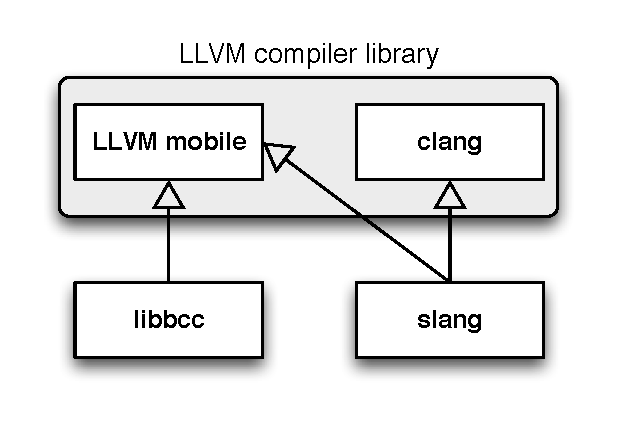
\includegraphics[scale=0.8]{fig/LLVMRef.eps}
    \caption{The referenece of LLVM compiler library}
    \label{fig:LLVMRef}
\end{center-figure}

To deploying \RRS{}, we have to back-port libbcc and libslang from Android Honeycomb to Gingerbread.

Five makefiles are modified for building the whole system:
\begin{enumerate}
    \item \verb|build/core/config.mk|
    \item \verb|build/core/definitions.mk|
    \item \verb|build/core/java.mk|
    \item \verb|build/core/package.mk|
    \item \verb|build/core/prelink-linux-arm.map|
\end{enumerate}

We brief the change as follows:
\paragraph{config.mk} sets up standard variables and other configuration like compiler flags.

\begin{lstlisting}[style=nonumbers]

SLANG := $(HOST_OUT_EXECUTABLES)/llvm-rs-cc$(HOST_EXECUTABLE_SUFFIX)
LLVM_RS_LINK := $(HOST_OUT_EXECUTABLES)/llvm-rs-link$(HOST_EXECUTABLE_SUFFIX)

ifeq ($(HOST_OS),darwin)
HOST_GLOBAL_CFLAGS += -arch i386
HOST_GLOBAL_CPPFLAGS += -arch i386
HOST_GLOBAL_LDFLAGS += -arch i386
endif

\end{lstlisting}

\paragraph{definitions.mk} mostly includes standard commands for building various types of targets, which are used by others to construct the final targes.
\begin{lstlisting}[style=nonumbers]
/**********************************************************
/* Find all of the RenderScript files under the named directories.
/*  Meant to be used like:
/*    SRC_FILES := $(call all-renderscript-files-under,src)
/**********************************************************/

define all-renderscript-files-under
$(patsubst ./%,%, \
   +  $(shell cd $(LOCAL_PATH) ; \
   +          find $(1) -name "*.rs" -and -not -name ".*") \
   +  )
endef

/**********************************************************
/* Commands to compile RenderScript
/***********************************************************/

define transform-renderscripts-to-java-and-bc
@echo "RenderScript: $(PRIVATE_MODULE) <= $(PRIVATE_RS_SOURCE_FILES)"
$(hide) rm -rf $(PRIVATE_RS_OUTPUT_DIR)
$(hide) mkdir -p $(PRIVATE_RS_OUTPUT_DIR)/res/raw
$(hide) mkdir -p $(PRIVATE_RS_OUTPUT_DIR)/src
$(hide) $(SLANG) \
    -o $(PRIVATE_RS_OUTPUT_DIR)/res/raw \
    -p $(PRIVATE_RS_OUTPUT_DIR)/src \
    $(foreach inc,$(PRIVATE_RS_INCLUDES),$(addprefix -I , $(inc))) \
    $(PRIVATE_RS_SOURCE_FILES)
    $(hide) $(LLVM_RS_LINK)    \
    $(PRIVATE_RS_OUTPUT_DIR)/res/raw/*.bc
    $(hide) mkdir -p $(dir $@)
    $(hide) touch $@
\end{lstlisting}

\paragraph{java.mk} takes charge of compiling .java files and .bc files.
\begin{lstlisting}[style=nonumbers]
###############################################################
## .rs files: RenderScript sources to .java files and .bc files
###############################################################
renderscript_sources := $(filter %.rs,$(LOCAL_SRC_FILES))
# Because names of the java files from RenderScript are unknown until the
# .rs file(s) are compiled, we have to depend on a timestamp file.
RenderScript_file_stamp :=
ifneq ($(renderscript_sources),)
renderscript_sources_fullpath := $(addprefix $(LOCAL_PATH)/, $(renderscript_sources))
RenderScript_file_stamp := $(LOCAL_INTERMEDIATE_SOURCE_DIR)/RenderScript.stamp

# prepend the RenderScript system include path
LOCAL_RENDERSCRIPT_INCLUDES := $(TOPDIR)frameworks/base/libs/rs/scriptc \
    $(LOCAL_RENDERSCRIPT_INCLUDES)

$(RenderScript_file_stamp): PRIVATE_RS_INCLUDES := $(LOCAL_RENDERSCRIPT_INCLUDES)
$(RenderScript_file_stamp): PRIVATE_RS_SOURCE_FILES := $(renderscript_sources_fullpath)
# By putting the generated java files into $(LOCAL_INTERMEDIATE_SOURCE_DIR), they will be
# automatically found by the java compiling function transform-java-to-classes.jar.
$(RenderScript_file_stamp): PRIVATE_RS_OUTPUT_DIR := $(LOCAL_INTERMEDIATE_SOURCE_DIR)/renderscript
# TODO: slang support to generate implicit dependency derived from "include" directives.
$(RenderScript_file_stamp): $(renderscript_sources_fullpath) $(SLANG)
   $(transform-renderscripts-to-java-and-bc)

LOCAL_INTERMEDIATE_TARGETS += $(RenderScript_file_stamp)
# Make sure the generated resource will be added to the apk.
LOCAL_RESOURCE_DIR := $(LOCAL_INTERMEDIATE_SOURCE_DIR)/renderscript/res $(LOCAL_RESOURCE_DIR)
endif

# source files generated from RenderScript must be generated before java compiling
ifneq ($(RenderScript_file_stamp),)
$(full_classes_compiled_jar): $(RenderScript_file_stamp)
endif

\end{lstlisting}

\paragraph{package.mk} includes standard rules for building an application package.
\begin{lstlisting}[style=nonumbers]
$(R_file_stamp): $(all_res_assets) $(full_android_manifest) $(RenderScript_file_stamp) $(AAPT) | $(ACP)
$(resource_export_package): $(all_res_assets) $(full_android_manifest) $($(RenderScript_file_stamp)) $(AAPT)
\end{lstlisting}

\paragraph{prelink-linux-arm.map} is a memory-mapping table for prelinking.
\begin{lstlisting}[style=nonumbers]
libbcc.so               0x99000000
\end{lstlisting}
    
%%%%%%%%%%%%%%%%%%%%%%%%%%%%%%%%%%%%%%%%%%%%%%%%%%%%%%%%%%%%%%%%%%%%
\section{slang}

\begin{enumerate}
    \item \textbf{Frontend}: Cleverly reuse Clang abstract syntax tree (AST) to reflect information back to Java layer.
    \item \textbf{Heavey-weight optimizations}: Bcc embeds metadata within bitcode (type, ...) to perform aggressive machine-independent optimizations on host before emitting portable bitcode.
    \item All bitcode supplied as a resource within .apk container.
\end{enumerate}


%%%%%%%%%%%%%%%%%%%%%%%%%%%%%%%%%%%%%%%%%%%%%%%%%%%%%%%%%%%%%%%%%%%%
\section{libbcc}

We shrink the size of LLVM by 10 times smaller to fit in a phone so that we could push frontend + heavy-weight optimizations to slang (in build time).
We do our own Execution engine and JIT, while just leveraging LLVM's low-level codegen libraries and have our 3 debugging mechanisms, so we just removed those big dwarf codes.

For a better Performance:
\begin{itemize}
    \item Fastcc calling convention
    \item VFPv3
    \item Use NEON instead of float4 
    \item Wide range of global, scalar optimizations
    \item 3x speedups over acc 
\end{itemize}
    
Libbcc design:
\begin{itemize}
    \item \textbf{Method-based JIT}: Reasonable scope for optimization.
    \item \textbf{Ahead-of-Time (AOT) compilation}: Caching of EXE cuts launch time.
    \item \textbf{Delta compilation}: Incremental compilation.
    \item \textbf{Modularity:} Each device will have its own JIT. For ARM devices, just include ARM codegen. Same thing for x86, PowerPC, mips devices.
    \item \textbf{On-device linking}: Specialization by CPU/GPU vendors.
    \item \textbf{Reflection}: Inter-operate across languages.
    \item \textbf{Portability}: Many languages target .bc and .bc targets many hardware.
\end{itemize}

%%%%%%%%%%%%%%%%%%%%%%%%%%%%%%%%%%%%%%%%%%%%%%%%%%%%%%%%%%%%%%%%%%%%
\section{LLVM for Android}
For reflection support, we have a tailored version of LLVM(Low Level Virtual Machine) for Android. LLVM\_mobile is ten times smaller than LLVM and three times faster\footnote{more for math-heavy code} than acc\footnote{old \RS{} compiler}.  

LLVM\_mobile is utilized as:
\begin{enumerate}
	\item \textbf{Disassembler} on the phone on the JIT results 	
	\item Android's \textbf{Self-Verifying Native JIT} ─ Three steps to eliminate the human assembler+emulator. First, using Disassembler to debug on assemble code. Second, comparing LLVM assemble code with GCC assemble code for locating where LLVM CodeGen bug is Solution. Third, use Anroid toolchain under prebuilt/ Also users libbcc.so, slang, and modified libElf for compare/verify. It's based on 3 assumptions: (1) Clang/LLVM compile the source and output correct .s; (2) Given a ".s", "as" generates correct binary; (3) ARM instructions can be read as a sequence of unsigned. %http://sourceware.org/bugzilla/show\_bug.cgi?id=11109. Also, other bugs on https://support.codesourcery.com/GNUToolchain/doc6300/getting-started.pdf.
 	\item Standalone \textbf{bcc} mocking RS apis ─ Determine whether a pair of statements is possible to access thread-shared data.
\end{enumerate}

%%%%%%%%%%%%%%%%%%%%%%%%%%%%%%%%%%%%%%%%%%%%%%%%%%%%%%%%%%%%%%%%%%%%
\section{Properties of Android Bitcode}

\begin{enumerate}
	\item ABI-level portability
	\item Basic types, structures and functions
    \item ILP32(Int, Long, and Pointer) , no LP64
    \item Data layout: \\
          \{i32, i32, i32\}: A triple of three i32 values\\
          \{float, i32 (i32) *\}: A pair, the second element is a pointer to a function that takes an i32, returning an i32
    \item Little endian
    \item A portable intermediate representation: \\
          .bc includes target triple in .bc, so runtime JIT can change it.\\
          .bc includes calling convention such as "Arm Architecture Procedure Call Standards"\\
          Bitcode didn't materialize it --> runtime JIT can change it
    \item Alignment: We don't use LLVM default alignments for space/time/GPU concerns. Alignment issues can't resort to runtime JIT, because code may have offsetof()
\end{enumerate}

\chapter{Conclusions and Future Work}
\label{c:conclusions}

After the demonstration of \Fountain{} in previous chapter, we know that the proposal of \RRS{} system is feasible and has a great extensibility. We summarize the advantages of \RRS{} as follows:
\begin{enumerate}
\item \textbf{Leveraging the hardwares on the remote engine} ─ Because \RS{} could do the computation and graphics operation, it's better to run on the more powerful hardwares. Unlike the other screen sharing mechanism, we fully exploit the power of the remote engine and relieve the network traffic. Only the RS command is necessary to send.
\item \textbf{No migration overhead} ─ The existing RS applications have almost no code necessary to be added or modified for migrating to \RRS{}. For instance, we migrate \Fountain{} without any overhead. Again, we are target for RS debugging framework, so the feature is important for \RRS{}.
\item \textbf{Debug for \RS{}} ─ \RRS{} speeds up the debugging progress no matter of using emulator or device. By punching through via \RRS{} and set up the environment, RS developer could have a better user experience on \RRS{} rather than the emulator. 
\end{enumerate}

%經過嚴密的測試之後,我們可以發現 RRS 這個框架的實作是一定可行的。而且有非常大的可擴充性,他有以下幾個好處:
%
%1. 充分的利用機器效能,效能表現不在受牽制於性能比較不可的程式
%因為 RS 同時可以繪圖與計算,不但需要強大的CPU 更需要強大的GPU,而往常的螢幕同步機制通常是把整個顯示在螢幕上的資訊壓縮然後整個傳輸過去,即使壓縮過後的 frame rate 可以提高,以會影響整個影像的品質,而我們不但可以充分的利用遠端引擎上的圖形硬體,還可以利用強大的計算能力,而不同的應用程式也會依其執行環境而擁有最佳表現。
%除此之外我們也讓網路的負擔最低,一旦把命令傳輸過去之後,就不再傳輸任何東西。
%
%2. 所有的應用程式不需要任何更動即可直接使用 RRS
%在 fountain 之中,我們沒有更動任何應用程式的程式碼,因為我們目標就是提供一個 framework,並且可以非常輕易的移植到 RRS 之上,這也是作為 debugger 所必要的一個特色。
%
%3. 解決 RS 沒有除錯機制的問題
%即使未來有了 emulator 支援了 open gl es 2.0 而可以跑 renderscript,因為整個是使用模擬出來的 arm (armv5),效能表現是相當差的,我們透過 RRS 間接的打穿,並且直接利用本機的圖形硬體加強了整體的效能表現。再透過 adb 設置好環境,就可以順利的江畫面傳送過去並進行除錯動作。
%
%4. 結合雲端應用的潛力
%除了除錯的應用以外,我們也在前面舉了相當多的例子,RS 未來最主要的應用或許是再遊戲,而現在手機非常普遍,未來多人連線「在地」遊戲或許會非常火紅,舉個例子來說,如果我們是完麻將遊戲,那麼麻將桌就是電視,電視連接四台手機,而每個手機則是自己的牌。透過 RRS 達成同步的機制,並且充分的各個手機的硬體效能,讓我們可以完美的實現三螢一雲,就如下圖,畫出我們整體的大方向。

\begin{center-figure}
	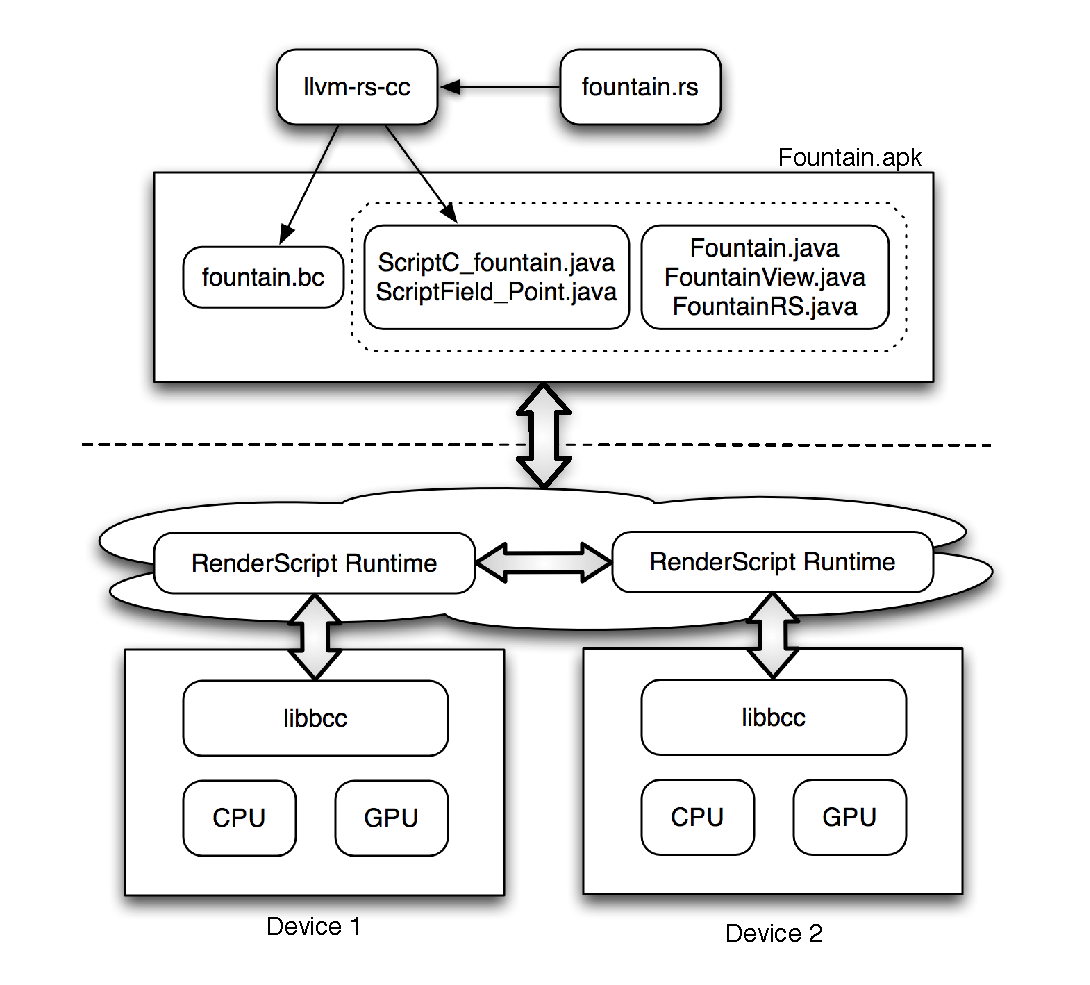
\includegraphics[scale=0.8]{fig/Future_RRS.eps}
	\caption{The big picture of Remote RenderScript}
	\label{fig:Future_RRS}
\end{center-figure}

It is just a \RRS{} prototype, there are still many stuff that we need work harder to perfect it in the future:

\begin{itemize}
\item \textbf{Heterogeneity among Devices} ─{} In the thesis, we just test \Fountain{} on the same devices. What if we communicate between two different devices? The size of screen might differ largely, e.g., smartphone and TV. Also, it must need a synchonization of screen size. We compute in individual devices, so we could scale the graphs up losslessly. The other easier approach is simply enlarging the window, but the resolution might be not satisfying. 
\item \textbf{Bi-directional Communication} ─{} One-way synchronization is not enough for non-debugging purposes. Our implementation is one-way by now, that is, one for sending and the other one for receiving only. In the future, we expect to extend it to have the ability of a two-way and one-to-many communication among devices. (As shown in Figure \ref{fig:StarCommunication} (a), and (b) respectively.) In other words, each device could be not only a client but also a server to facilitate our desirable personal-cloud.
\item \textbf{Application for Cloud Computing} ─{} As we said in Chapter \ref{c:intro}, gaming might are the main purpose of \RS{}. Of course, \RRS{} is suitable for game development. For instance, everyone might have one smartphone in the recent future. Game vendor could use \RRS{} to develop a multi-player game instread of tranditional board games, and replace the board with a larger screen device like TV. Our vision is similar with Google Project Tungsten.
\item \textbf{Security} ─{} Network pairing must be done to set up the environment for \RRS{}. For security concern, auto-pairing is not permitted. So the authentication is necessary in the future network-pairing process to eliminate security concern.
\end{itemize}


\begin{center-figure}
	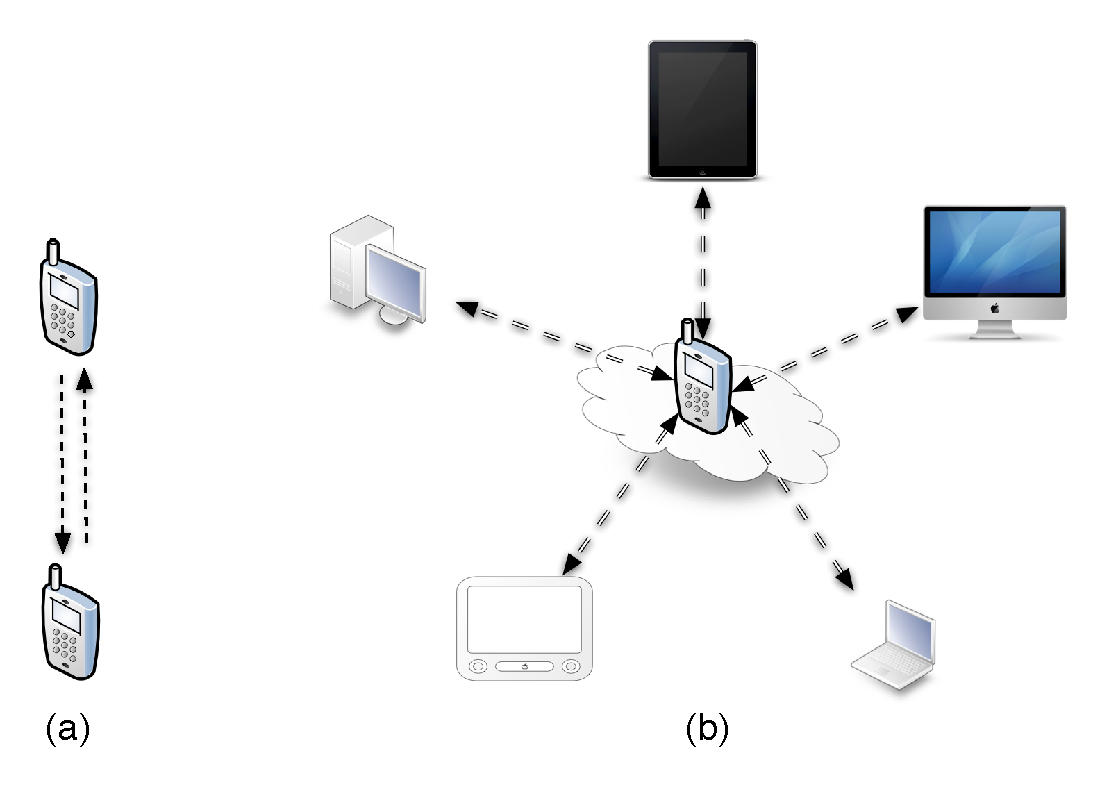
\includegraphics[scale=0.8]{fig/NetworkCommunication_Star.eps}
	\caption{Communication among hetrogeneous devices: (a) Bi-Direction (b) One-to-Many}
	\label{fig:StarCommunication}
\end{center-figure}
%1. Should we scle up when the remote has larger screen?
%目前我們測試是在兩隻相同的手機之上,但是如果未來是再不同裝置之間傳送,螢幕大小的差距可能會非常的大,例如手機與電視,那我們勢必要加上螢幕的同步處理,因為我們只是個指令,所以或許可以直接透過指令去分析,並且做不失真的圖形放大處理。另外一種比較簡單的作法就是單純的裝置上實作最大化視窗的功能,但是可能解析度的表現就不如上述方法還好。
%
%2. two-way synchronization
%如果要將 RRS 使用再非除錯的用途之上,單方向的傳送勢必是不足的,而目前我們的實作之中,只純粹的處理單方向同步,也就是 client-server 單一架構,未來的話,預計將其擴展,每個裝置本身同時可以是 server 也可以是 client,實現所謂的 personal-cloud 理想。
%
%3. Authentacation
%每個裝置連線時,我們必須事先做好網路pairing 的工作,但是我們不可以允許自動的配對,這會有安全性上的問題,所以未來如果我們要使用RRS 再一般應用之上(例如遙控播放),那麼我們就必須在其之上加入認證機制,解決安全性上的問題。

%--
%2. need to sync, should implement a network flush()
%cmd+1 is only if (dataLen < DATA\_SYNC\_SIZE), we should take care of other cases
%從前面我們可以了解到指令分為需要同步與不需要同步兩種,而在 Fountain 中,其需要的指令都是不必同步的,所以我們日後勢必還得處理同步問題。
%
%4. Now we only handle ScriptInvokeV(...). In other functions, there are must some pointer in the parameters (inconsistent memory addr).
%雖然整體來說需要傳送的指令種類不多,但是因為每個指令的參數都不一樣,而這種不同的參數都必須處理其記憶體位址問題,所以如果未來要將RRS 擴展,勢必也要將其他函式的問題解決
%
%5. Because ScriptCCreate is luckily the last "Create" command, we could get the pointer from mToCoreRet directly.
%--






\backmatter

\addcontentsline{toc}{chapter}{\bibname}
\bibliographystyle{abbrv}

% input your reference here
\bibliography{thesis,other}

\appendix
%\chapter{Example of Graphs in Static Data Race Detector}
\label{c:appendix_A}

This appendix shows how the graph is transformed in our presented static data detector for OpenMP programs. Given an example shows in \reflst{l:omptsa-example-program}, 

\begin{lstlisting}[caption={Example program},label={l:omptsa-example-program}]
	void SFFT (int A[], int N) {
		int i;
		const int half = N / 2;
		
		if (half == 1)	// base case for recursion
			return;
			
		#pragma omp parallel
		{
			#pragma omp single task
			{
				#pragma omp task
				SFFT(A, half);
				#pragma omp task
				SFFT(A + half, half);
				#pragma omp taskwait
			}
		}
		
		#pragma omp for nowait
		for (i = 0; i < half; i++) {
			// Just do something for A[i] and A[i + half]
			A[i] += i;
			A[i + half] += i + half;
		}
	}
\end{lstlisting}


\end{document}
